\documentclass[]{article}
\usepackage{lmodern}
\usepackage{amssymb,amsmath}
\usepackage{ifxetex,ifluatex}
\usepackage{fixltx2e} % provides \textsubscript
\ifnum 0\ifxetex 1\fi\ifluatex 1\fi=0 % if pdftex
  \usepackage[T1]{fontenc}
  \usepackage[utf8]{inputenc}
\else % if luatex or xelatex
  \ifxetex
    \usepackage{mathspec}
  \else
    \usepackage{fontspec}
  \fi
  \defaultfontfeatures{Ligatures=TeX,Scale=MatchLowercase}
\fi
% use upquote if available, for straight quotes in verbatim environments
\IfFileExists{upquote.sty}{\usepackage{upquote}}{}
% use microtype if available
\IfFileExists{microtype.sty}{%
\usepackage{microtype}
\UseMicrotypeSet[protrusion]{basicmath} % disable protrusion for tt fonts
}{}
\usepackage[margin=1in]{geometry}
\usepackage{hyperref}
\hypersetup{unicode=true,
            pdftitle={Ornaments as indicators of social changes and cultural practices in northeastern Taiwan before and after European colonial period},
            pdfauthor={Li-Ying Wang; Ben Marwick},
            pdfkeywords={Historical archaeology; Iron Age; European colonisation; Trade
ornaments; Exchange networks; Taiwan; Monte Carlo simulation},
            pdfborder={0 0 0},
            breaklinks=true}
\urlstyle{same}  % don't use monospace font for urls
\usepackage{graphicx,grffile}
\makeatletter
\def\maxwidth{\ifdim\Gin@nat@width>\linewidth\linewidth\else\Gin@nat@width\fi}
\def\maxheight{\ifdim\Gin@nat@height>\textheight\textheight\else\Gin@nat@height\fi}
\makeatother
% Scale images if necessary, so that they will not overflow the page
% margins by default, and it is still possible to overwrite the defaults
% using explicit options in \includegraphics[width, height, ...]{}
\setkeys{Gin}{width=\maxwidth,height=\maxheight,keepaspectratio}
\IfFileExists{parskip.sty}{%
\usepackage{parskip}
}{% else
\setlength{\parindent}{0pt}
\setlength{\parskip}{6pt plus 2pt minus 1pt}
}
\setlength{\emergencystretch}{3em}  % prevent overfull lines
\providecommand{\tightlist}{%
  \setlength{\itemsep}{0pt}\setlength{\parskip}{0pt}}
\setcounter{secnumdepth}{0}
% Redefines (sub)paragraphs to behave more like sections
\ifx\paragraph\undefined\else
\let\oldparagraph\paragraph
\renewcommand{\paragraph}[1]{\oldparagraph{#1}\mbox{}}
\fi
\ifx\subparagraph\undefined\else
\let\oldsubparagraph\subparagraph
\renewcommand{\subparagraph}[1]{\oldsubparagraph{#1}\mbox{}}
\fi

%%% Use protect on footnotes to avoid problems with footnotes in titles
\let\rmarkdownfootnote\footnote%
\def\footnote{\protect\rmarkdownfootnote}

%%% Change title format to be more compact
\usepackage{titling}

% Create subtitle command for use in maketitle
\providecommand{\subtitle}[1]{
  \posttitle{
    \begin{center}\large#1\end{center}
    }
}

\setlength{\droptitle}{-2em}

  \title{Ornaments as indicators of social changes and cultural practices in
northeastern Taiwan before and after European colonial period}
    \pretitle{\vspace{\droptitle}\centering\huge}
  \posttitle{\par}
    \author{Li-Ying Wang \\ Ben Marwick}
    \preauthor{\centering\large\emph}
  \postauthor{\par}
      \predate{\centering\large\emph}
  \postdate{\par}
    \date{11 December, 2019}


\begin{document}
\maketitle
\begin{abstract}
Long-lasting indirect impacts on indigenous peoples in the periphery of
colonial control are poorly understood, especially in East Asia. Trade
ornaments from Kiwulan (1400-1900 AD) in northeastern Taiwan show the
indirect impacts of European colonial activities on local societies. The
diversity of ornaments was greater during the period of European
presence compared to previous periods, and their spatial distribution
was more clustered. This hints at increasing social inequality resulting
from a colonial influence. Ornaments give insights into the increasing
social inequality stimulated by European colonisation, and show the
agency of indigenous people to incorporate ornaments into their social
system.
\end{abstract}

\hypertarget{introduction}{%
\section{Introduction}\label{introduction}}

The direct impacts of European colonialism on indigenous communities in
East Asia were much less conspicuous than in island Southeast Asia and
Oceania. Direct European colonial rule throughout East Asia was rare and
limited, and the question of long-lasting indirect impacts on local
indigenous communities remains largely unanswered. Understanding the
indirect effects of colonialism are important for detecting colonial
impacts on indigenous peoples in the periphery of colonial control
(Trabert 2017). In many parts of the world, the introduction of foreign
trade goods by colonial traders into local indigenous societies caused
substantial transformations of indigenous economic, cultural, and
socio-political systems (Dietler 2005; Dietler 1997; Junker 1993;
Silliman 2005). Consumption patterns of foreign goods can give insights
into negotiations between colonized and colonizer, and the resistance
and accommodations of indigenous people through their daily cultural
practices (Dietler 2015; Given 2004; Mullins 2011; Scaramelli \&
Scaramelli 2005; Silliman 2001; Torrence \& Clarke 2000; Voss 2005).
Northeastern Taiwan is an ideal context to study peripheral colonial
influence because although there was a prominent Spanish and Dutch
colonial presence in parts of Taiwan, the northeastern region was
isolated from intensive direct contact by the Xueshan Mountains.

This article describes personal ornaments excavated from the upper
component of Kiwulan (1400 AD-1900 AD), the largest Iron Age settlement
on the Yilan plain in northeastern Taiwan. The first recorded European
presence in Yilan was a Spanish revenge attack on indigenous villages in
1632 (Borao 2001: 163). In 1647 the Dutch attacked villages and forced
them to accept colonial rules and pay an annual tribute (Andrade 2007).
According to Dutch census reports in 1650, Kiwulan was the largest
indigenous settlement in the plain, with a population of 840 adults
(Nakamura 1938: 12). Following defeat of Dutch by the Chinese general
Koxinga in 1661-1662, the Dutch abandoned northern Taiwan. Direct
contact with Han Chinese is indicated by Qing dynasty census reports
mentioning Yilan villages in 1821 (Yao 1996).

One of the most commonly traded types of object in this region were
ornaments such as glass and stone beads (Chen 2007; Li \& Chiu 2014;
National Musuem of Taiwan History 2005). Personal adornments in the
archaeological record are useful as signal of an individual's status
(Joyce 2005; Scaramelli \& Scaramelli 2005). The consumption of stone
beads in Southeast Asia during Iron Age is often associated with
increasing social stratification or socio-political complexity (Bellina
2014; Carter 2016; Francis 2002; Theunissen \emph{et al.} 2000; Kenoyer
2000). In this paper, we explore archaeological ornaments from Kiwulan
spanning the pre-European contact period, the period of Spanish and
Dutch presence, and the following period of Chinese presence. We address
the question of whether indirect colonial influences on the indigenous
populations can be detected through the ornament assemblages.

\hypertarget{ornaments-in-complex-exchange-network-during-the-late-iron-age-and-early-historical-period}{%
\section{Ornaments in complex exchange network during the late Iron Age
and early historical
period}\label{ornaments-in-complex-exchange-network-during-the-late-iron-age-and-early-historical-period}}

The island of Taiwan lies at the junction of mainland China, Southeast
Asia, and Northeast Asia in the Pacific Ocean. The prehistory of Taiwan
island could be roughly divided into three major periods, paleolithic
(c.~27,000 BP- 5000BP), Neolithic (c.~6500- 2000BP), and Iron age
(c.~2000- 400BP) with slightly regional differences in onset of each
period and variations in style of artifacts and assemblages (Liu 2011;
Chen 2017). It is generally accepted that Taiwan entered the historical
period in the early 17th century due to the colonial activities of the
Spanish and the Dutch who played an important role in keeping written
records about Taiwan. The European colonial presence in Taiwan ended in
1662 when the Dutch were defeated by the kingdom of Tungning, founded by
Koxinga from China. Later in 1683, Taiwan was incorporated into the Qing
dynasty in China and a large wave of Han Chinese migrated to Taiwan
during the late 18th century. Because of natural safe harbors, northeast
Taiwan was involved in a regional trade network through cross-culture
interactions with Chinese merchants since the 14th century, and later
the global trade network with the Europeans in the 17th century brought
more trade goods circulated in Southeast Asia into Taiwan (Chen 2005;
Liu \& Wang 2017). Although located on the periphery of regional trade
centers, Yilan was connected to trade networks via visits of other
indigenous groups, Chinese merchants, and Europeans, via sea.

The European presence in northern Taiwan started with the Spanish who
founded Fort San Salvador at Keelung in 1626, and Fort San Domingo in
1629 at Tamsui. They sent missionaries to local indigenous settlements
in this region (Blussé \& Everts 2000: 343) and kept records about their
observations of indigenous communities. A Dominican priest in 1632
reported that the Taparri, an indigenous tribe from northern Taiwan,
exchanged carnelian beads with other indigenous groups. This form of
exchange was widespread and even the Spanish soldiers used carnelian
beads as bargaining chips for gambling (Li \& Wu 2006: 132--49). The use
of beads as prestige goods is further indicated by their role in bride
price payments, and compensation to resolve disputes (Li \& Wu 2006:
132--49). Other records mention that the female shamans in the tribe
would use carnelian beads as magical items in ritual healing practices
(Borao 2009: 122--51). Records of an indigenous funeral document the use
of carnelian beads in ritual contexts, with more carnelian beads,
pottery, and cloth placed into the graves of more influential people to
indicate their family's higher status (Li \& Wu 2006: 153). While a full
critical analysis of these historical accounts remains to be produced,
we take them to minimally indicate that carnelian beads were already
treated as prestige goods in Yilan before the arrival of Europeans. In
1642, the Dutch Vereenigde Oostindische Compagnie (VOC) defeated the
Spanish and took over their forts in northern Taiwan. They introduced a
feudal system in an attempt to control the indigenous communities by
asking indigenous leaders to attend an annual ceremony for demonstrating
their loyalty and paying tributes (Andrade 2007, ch.~9; Kang 2016,
ch.~4). The Dutch provided beads and other goods based on negotations
with indigenous communities to secure alliances in the annual ceremony
or during travelling (Kang 2016, ch.~6). We might predict that the
activities of the Dutch feudal system to build and maintain alliances
resulted in an increase in the amount and diversity of ornaments in
northeastern indigenous communities during this period.

Chinese historical records from 1829, 1837, and 1852 during the Qing
dynasty (1616-1911) contain some notes on the purposes of ornaments from
Yilan (Chen 1963: 228, 308; Ke 1993: 11, 126; Yao 1996: 77). According
to those records, indigenous people in Yilan wore ornaments in
ceremonial contexts to display their wealth and status. Among those
ornaments, fish-shaped necklaces made of metal threads had high value
due to their delicacy and the exotic materials invested in production.
These were usually possessed by wealthy people. Other people wore
carnelian beads or glass beads on their head or neck to participate in
ceremonies. In 1895, at the beginning of Japanese colonisation, an
academic field survey for plains indigenous groups reported that
fish-shaped metal necklaces necklaces were not used in Yilan at that
time, but elderly people still used beads (Ino 1996: 227--32). Although
these historical records are fragmentary and may contain some biases
(Galloway 2006) that have not yet been studied in detail, we find
consistency among multiple sources in their descriptions of how
ornaments represent high status or specialised social roles in
indigenous communities in Yilan. Compared to the European period, there
are fewer documentary mentions of beads in the Chinese period and the
descriptions are limited to clothing, but these generally confirm the
role of beads as status markers.

Ornaments found in northeastern Taiwan in the early historical period,
including glass beads, stone beads, and metal ornaments, are considered
to have been imported from other regions. This is because of to a lack
of archaeological evidence of beadmaking waste, metalworking, or
accessible local raw materials. The chemical composition of glass beads
from this region shows a high content of lead and, toghether with the
winding/folding technique, these details suggest a Chinese beadmaking
tradition (Cheng 2008; Gan \emph{et al.} 2006; Wang 2018). Although
there is a wide variety of metal ornaments such as bells, bracelets,
rings, and pendants, the common components of metal ornaments are brass
and copper, with a small number made from lead and tin that indicates
multiple origins that include Southeast Asia (Chen 2011). There is no
direct evidence showing European delivery of beads, however, a large
amount of the glass beads containing gold foil (hereafter, gold-foil
beads) at Kiwulan might have been introduced by the Spanish through
economic activities because similar beads were found at Luzon, northern
Philippines, as part of the trading route of the Spanish between 16-19th
century (Wang \& Liu 2007). Both archaeological evidence and historical
records indicate northeastern Taiwan was involved inregional networks
with East Asia in the late Iron age. These included Chinese merchants
trading metal items, clothes, and beads with local indigenous people in
Taiwan in exchange for local resources. The foreign-made large dark
brown glazed stoneware jars frequently found in European shipwrecks were
also commonly found from many sites in Taiwan, suggesting direct or
indirect interactions. Despite the Chinese origin of some ornaments at
Kiwulan, there is compelling evidence that a large amount of ornaments
found at 17th century sites resulted from European colonial and economic
activities in the region.

\hypertarget{excavations-at-kiwulan-in-northeastern-taiwan}{%
\section{Excavations at Kiwulan in northeastern
Taiwan}\label{excavations-at-kiwulan-in-northeastern-taiwan}}

\begin{figure}
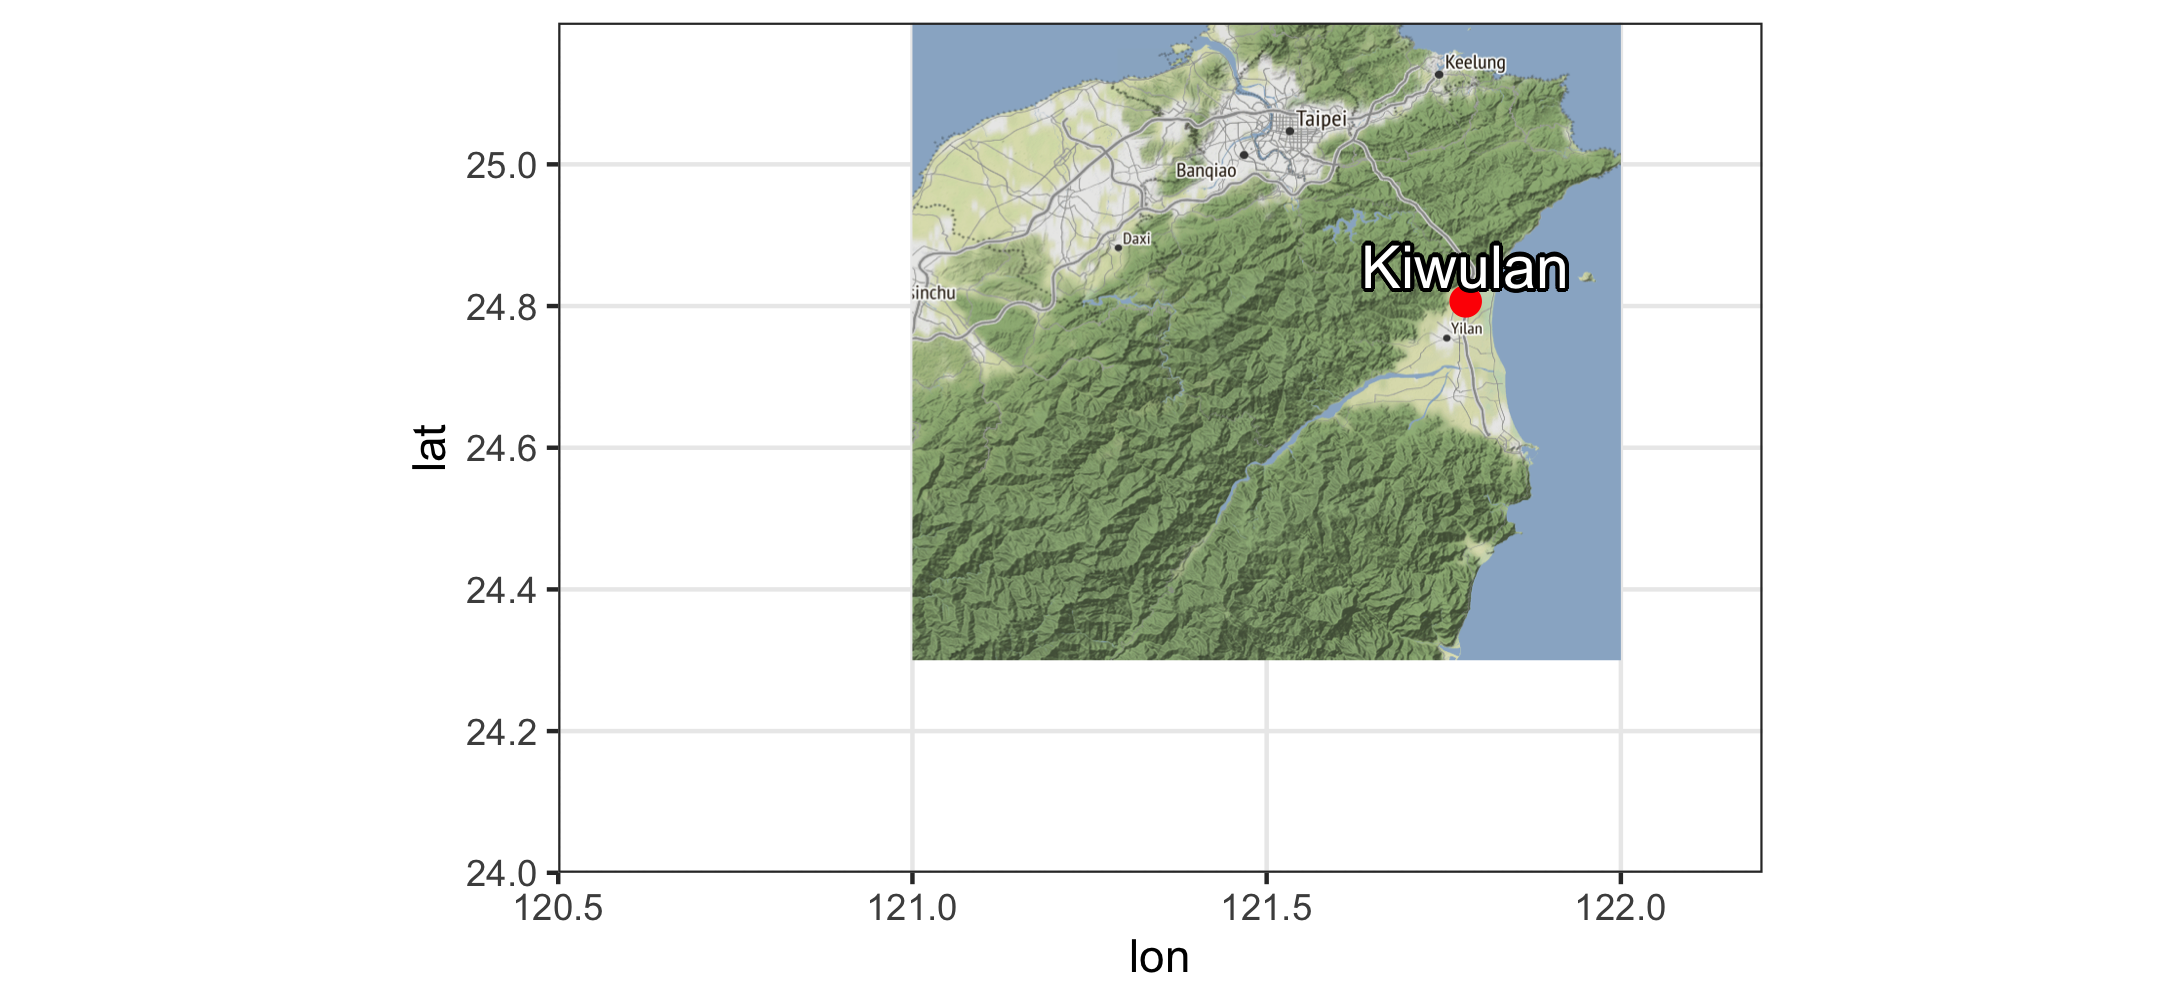
\includegraphics[width=5.31in]{/Users/bmarwick/Desktop/kwl-ornaments/analysis/figures/kiwulan-location-map} \caption{Map showing the location of Kiwulan, and other places in northern Taiwan named in the text. Map data from naturalearthdata.com}(\#fig:KWL-map)
\end{figure}

\begin{figure}
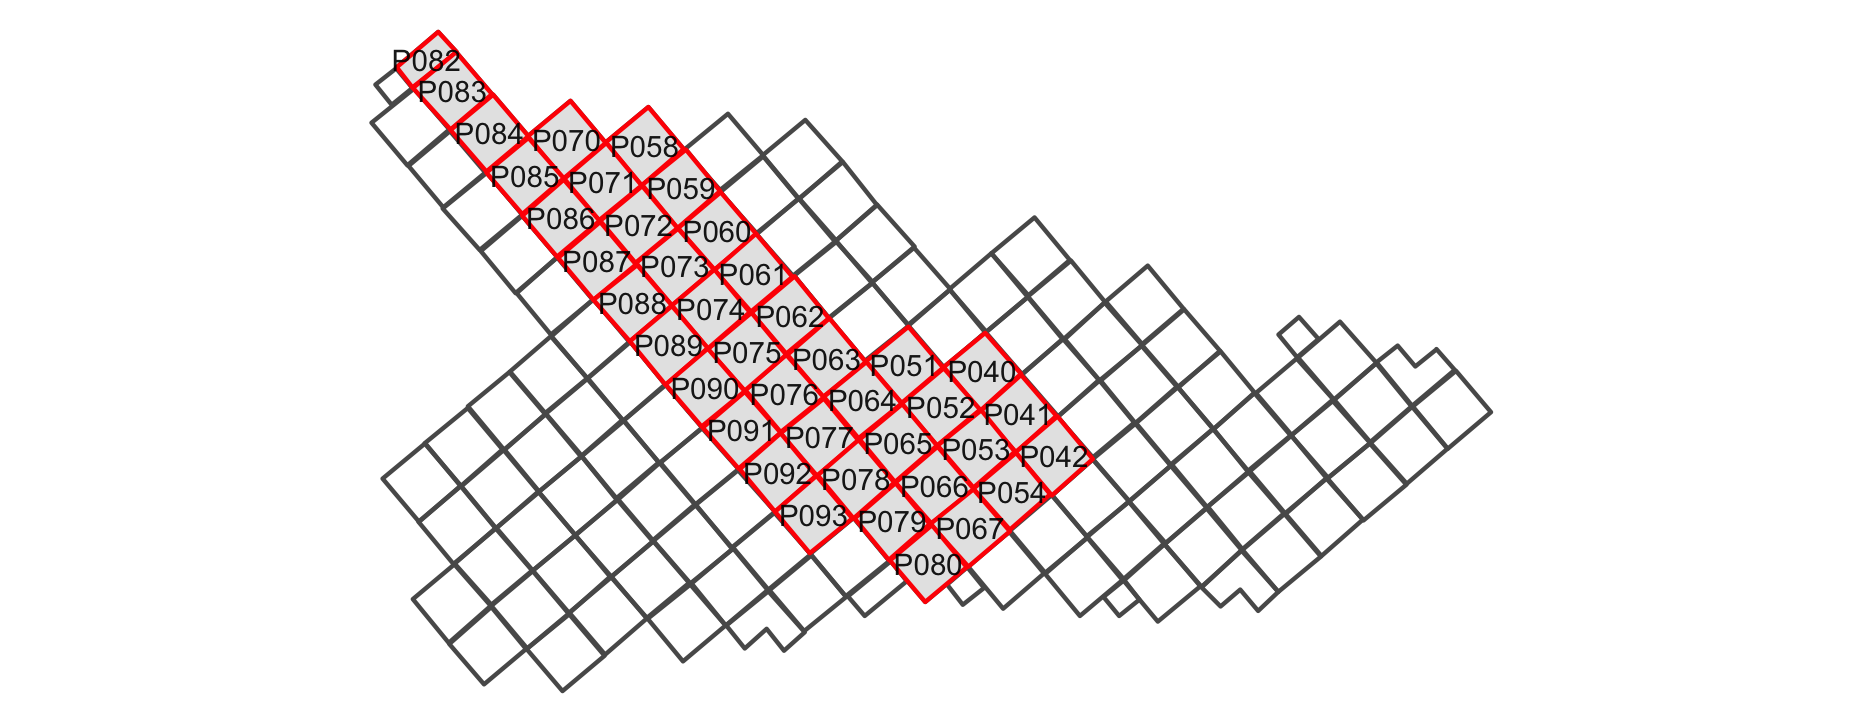
\includegraphics[width=5.31in]{/Users/bmarwick/Desktop/kwl-ornaments/analysis/figures/KWL-excavation-map} \caption{Map showing the largest section of excavation areas at Kiwulan, and the distribution of forty squares sampled in this paper presented in red with square ID number. Small dots represent the location of post-holes. Each square is 4 x 4 m}(\#fig:KWL-sam-area)
\end{figure}

Information about Kiwulan (Figure @ref(fig:KWL-map)) comes from a rescue
archaeology project that during 2001-2004 in advance of a water
diversion project and road bridge construction. The excavations used 2
mm and 1.5 mm mesh screens and covered eight open area sections in total
of 262 squares (4 m by 4 m) reaching 3,814 m\textsuperscript{2} (Chen
2007). The nearly 2 m thick archaeological deposits reveal a large
amount of artefacts, burials, middens, post-holes, wooden pillars, and
stone structures, all of which indicates it was a long-term settlement.
Artefact locations were recorded to the 2 x 2 m sub-square they were
recovered in; they lack individual point provenance. Based on the
continuity of deposition and the frequency of artifacts, the center of
the site is the open area consisting of A and D sections, which is also
the study area where our samples selected from. In the AD area,
post-holes were found aligned in a north-south direction in some
intervals with construction marks, which were interpreted as the remains
of silt house structures. At the north margin of the dwelling place were
burials that are mostly oriented in an east-west direction (Figure
@ref(fig:KWL-sam-area)).

The chronology of Kiwulan can be divided into two phases represented by
a upper component (1400-1900 AD, 600-100 BP) and a lower component
(700-1200 AD, 1200-800 BP) separated by a sterile deposit spanning
c.~150 years. These component divisions are based on the differences in
the colour and texture of the deposit. The interpration of the sterile
deposit is still under debate, with pollen analysis suggesting dry
weather leading to site abandonment (Lin 2015; Chiu 2004; Chen 2007).
There are 32 radiocarbon ages spanning the two components, previously
published by Chen (2007), and shown here in Figure @ref(fig:C14-data)
and Table @ref(tab:C14-table-data). We focus on the upper component
because only this componant spans the periods of pre-European contact,
European presence, and Chinese presence. In the upper component, all
excavation squares in our sampling area show signs of continuous human
occupation during each of the three phases. Previous work divided the
upper component into six analytical units, spanning from the 14th
century to the 19th century, according to the radiocarbon dates,
excavation depth, consistency of contexts, and types of chronologically
diagnostic ceramics such as blue and white porcelains (Hsieh 2009; Wang
2011). However, we found some ambiguities in the previous chronology, so
to help answer our research question, we re-examined the upper component
to devise a new chronology to assign artefacts to the pre-European,
European, and the Chinese periods.

The archaeological indicators of the start of the European influence at
Kiwulan are the appearance of light grey glazed jars, known as
``An-ping'' jars in China and Taiwan, and large dark brown glazed
stoneware jars that were introduced to Taiwan during the early 17th
century. Large dark brown glazed stoneware jars may have been made in
Southeast Asia, and are frequently found in European shipwrecks from
this period as vessels for transporting water, wine or other liquids on
long voyages. The earliest evidence oflight gray glazed jars in this
region has been found among the cargo of the Spanish shipwreck \emph{San
Diego}, which sunk in 1600 AD (Hsieh 2009; Hsieh 1995). Southeast China
is assumed to be the origin of the light gray glazed jars, however these
are commonly found at sites in Taiwan that were associated with European
activities, such as the Zeelandia fort site in Tainan (Wang \& Liu
2007). The jar shapes found at Kiwulan are typical of those found
elsewhere in VOC sites occupied during the 17th century (Berrocal
\emph{et al.} 2018: 917; Cort 2017: 282; Grave \& McNiven 2013; Ketel
2011; Klose \& Schrire 2018: 131). We cannot be sure of the exact
process that bought them to Kiwulan: they might have been directly
imported by Europeans, by Chinese merchants, or by indigenous groups via
regional networks in north Taiwan. In any case, the high volume of
ceramics transported by Europeans, and their high mobility in shipping
trade played an important role in introducing foreign jars to Taiwan.
Those jars were widely distributed across the site and can serve as
indicators, together with the radiocarbon dates, to identify the
excavation units associated with the pre-European period and the start
of European influence at Kiwulan. In addition to stoneware jars as
indicators of European presence, around 300 pieces of locally made pipes
and a few imported pipes were found at Kiwulan. Smoking is likely to
have been introduced by Europeans, and we found that the presence of
pipes in the archaeological record here is consistent with distributions
of glazed jar fragments, which are far more numerous and widespread
across the site (n = 1685).

The archaeological signature of the Chinese period at Kiwulan is the
large amount and diversity of Chinese porcelains in many forms such as
bowls, plates, and cups. Other indicators include opium pipe-bowls and
distinctive architectural bricks and tiles used by Chinese (Hsieh 2009).
Chinese migrations to Yilan were also recorded in official Chinese
records written in the early 19th century recording the first immigrants
in 1768 (Chen 1963; Ke 1993).

\begin{figure}
\centering
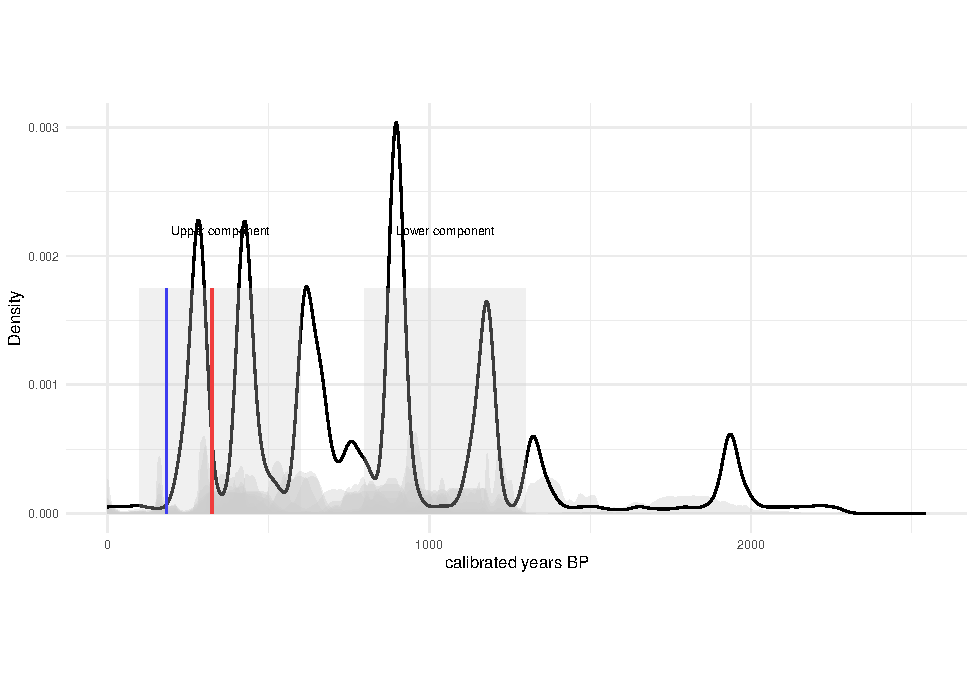
\includegraphics{../figures/C14-data-1.pdf}
\caption{(\#fig:C14-data)Summed probability distributions for dates from
Kiwulan. The dark line represents the summed probabilities of all
radiocarbon ages, and the grey lines in the background are the
probabilities of individual ages. Grey rectangles indicate the
approximate chronology of the major archaeological components of the
deposit. For the upper component, the blue line indicates the start of
European presence, while the red line is the Chinese presence. Ages
calibrated with the Bchron package (Parnell et al.~2008).}
\end{figure}

\begin{table}

\caption{(\#tab:C14-table-data)Radiocarbon dates on charcoals from Kiwulan (Chen 2007). Calibrated using IntCal13 Atmospheric curve. In the context column, original numbering system from excavation report is used, such M009 means burial No.9 }
\centering
\begin{tabular}[t]{l|l|l|l|l|l}
\hline
Lab code & Pit-Layer & Above mean sea level (cm) & Date BP & Calibrated date (95\% conf. level) & Context\\
\hline
NTU-3803 & P052-L7 & 0 to -10 & <200yr &  & artefact-bearing deposit\\
\hline
NTU-3925 & P051-L17 & -36 to -56 & <200yr &  & sterile deposit\\
\hline
NTU-3943 & P051-L19 & -70 to -90 & <200yr &  & sterile deposit\\
\hline
NTU-4283 & P063-L12 & -30 to -70 & <200yr &  & midden, H044\\
\hline
NTU-4293 & P089-L11 & -50 to -70 & <200yr &  & artefact-bearing deposit\\
\hline
NTU-4305 & P089-L7 & -20 to -30 & <200yr &  & artefact-bearing deposit\\
\hline
NTU-4322 & P051-L11 & 0 to -40 & <200yr &  & midden, H026\\
\hline
NTU-4323 & P070-L3 & 20 to -57 & <200yr &  & burial, M095\\
\hline
NTU-3993 & P041-L7 & -25 to -45 & 250±40 & 4-431 & artefact-bearing deposit\\
\hline
NTU-4419 & P162-L3 & -10 to -110 & 280±70 & 11-485 & midden H172\\
\hline
NTU-4311 & P052-L16 & -110 to -130 & 310±100 & 17-510 & artefact-bearing deposit\\
\hline
NTU-4320 & P168-L1 & 6 to -51 & 340±100 & 38-528 & midden, H193\\
\hline
NTU-4016 & P028-L9 & -44 to -80 & 270±40 & 145-453 & burial, M020\\
\hline
NTU-4310 & P018-L2 & -28 to -70 & 360±100 & 73-542 & burial, M039\\
\hline
NTU-3791 & P049-L11 & -20 to -30 & 340±30 & 314-482 & artefact-bearing deposit\\
\hline
NTU-4292 & P052-L6 & 4 to -56 & 510±75 & 344-648 & burial, M009\\
\hline
NTU-4304 & P066-L11 & -40 to -60 & 600±75 & 515-675 & artefact-bearing deposit\\
\hline
NTU-4423 & P144-L5 & -10 to -30 & 610±90 & 504-709 & artefact-bearing deposit\\
\hline
NTU-4315 & P248-L5 & -100 to -120 & 800±120 & 560-950 & artefact-bearing deposit\\
\hline
NTU-3926 & P041-L9 & -70 to -90 & 900±50 & 714-917 & sterile deposit\\
\hline
NTU-4421 & P162-L11 & -160 to -180 & 920±70 & 706-954 & artefact-bearing deposit\\
\hline
NTU-4319 & P154-L3 & 10 to -10 & 920±105 & 685-1053 & artefact-bearing deposit\\
\hline
NTU-4430 & P238-L10 & -130 to -150 & 1020±60 & 796-1055 & sterile deposit\\
\hline
NTU-4422 & P237-L4 & -70 to -90 & 1030±80 & 779-1156 & artefact-bearing deposit\\
\hline
NTU-3788 & P028-L15 & -130 to -150 & 1050±40 & 891-1050 & artefact-bearing deposit\\
\hline
NTU-4428 & P154-L13 & -170 to -180 & 1080±90 & 802-1222 & artefact-bearing deposit\\
\hline
NTU-4427 & P246-L8 & -160 to -180 & 1170±70 & 956-1255 & artefact-bearing deposit\\
\hline
NTU-4316 & P019-L5 & -100 to -120 & 1190±70 & 969-1263 & burial, M066\\
\hline
NTU-3792 & P041-L13 & -150 to -170 & 1240±30 & 1079-1261 & artefact-bearing deposit\\
\hline
NTU-4434 & P144-L11 & -130 to -150 & 1480±70 & 1292-1524 & artefact-bearing deposit\\
\hline
NTU-4321 & P154-L14 & -180 to -190 & 1870±110 & 1561-2085 & artefact-bearing deposit\\
\hline
\end{tabular}
\end{table}

\hypertarget{the-personal-ornaments}{%
\section{The personal ornaments}\label{the-personal-ornaments}}

\begin{figure}
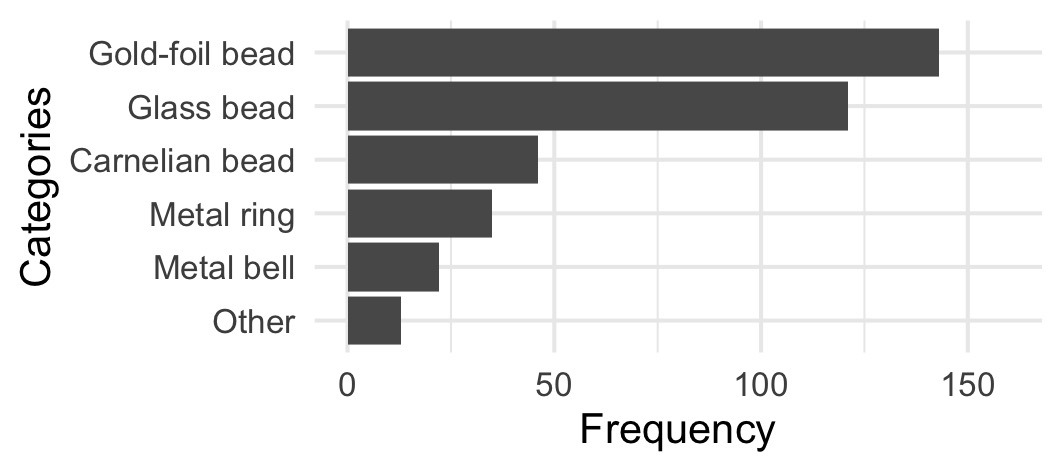
\includegraphics[width=3.54in]{/Users/bmarwick/Desktop/kwl-ornaments/analysis/figures/plot-ornaments-count} \caption{Frequency of the major class of ornaments at Kiwulan. Frequency represents artefact counts}(\#fig:plot-all-ornaments-count)
\end{figure}

\begin{table}

\caption{(\#tab:tidy-data-for-table)Ornament subtype at Kiwulan. The numbers represent artefact counts }
\centering
\begin{tabular}[t]{l|l|r|r|r}
\hline
Categories & Type & Before European Contact & European Presence & Chinese Presence\\
\hline
Agate bead & hexagonal & 6 & 17 & 5\\
\hline
Agate bead & waxy oval & 0 & 4 & 0\\
\hline
Agate bead & small oval & 3 & 3 & 0\\
\hline
Agate bead & globular & 0 & 1 & 0\\
\hline
Agate bead & pentagonal & 0 & 1 & 0\\
\hline
Agate bead & big oval & 0 & 0 & 1\\
\hline
Agate bead & long bicone & 0 & 0 & 1\\
\hline
Agate bead & octagonal & 0 & 0 & 1\\
\hline
Bell & large & 3 & 8 & 3\\
\hline
Bell & plain small & 0 & 4 & 1\\
\hline
Bell & thin small & 0 & 1 & 1\\
\hline
Glass bead & small (0.5-1 cm) & 60 & 37 & 1\\
\hline
Glass bead & medium (1-2 cm) & 8 & 15 & 0\\
\hline
Golden bead & NA & 48 & 93 & 2\\
\hline
Metal ring & wide small & 1 & 9 & 1\\
\hline
Metal ring & thin large & 4 & 5 & 2\\
\hline
Metal ring & wide large & 0 & 5 & 0\\
\hline
Metal ring & overlapped & 0 & 2 & 0\\
\hline
Metal ring & braid & 0 & 1 & 0\\
\hline
Metal ring & entwined & 1 & 1 & 0\\
\hline
Metal ring & flat & 0 & 1 & 0\\
\hline
Metal ring & large thick string & 0 & 1 & 0\\
\hline
Metal ring & small thin string & 0 & 1 & 0\\
\hline
\end{tabular}
\end{table}

\begin{figure}
\includegraphics[width=5.93in]{/Users/bmarwick/Desktop/kwl-ornaments/analysis/figures/ornament} \caption{Subtypes of ornament in each major class. A: carnelian beads, B: bells, C: glass beads and gold-foil beads, D: metal rings. Photographs are presented in the same order as those subtypes in the table but from left to right instead. The photographs of B, C, D classes were from original excavation report (Chen 2007).}(\#fig:ornaments-image)
\end{figure}

Ornaments were found in a variety of archaeological contexts including
post-holes area, burials, and middens. This study focuses on 406
ornaments from 40 sampling squares located at the dwelling place of
Kiwulan, indicated by aligned post-holes with \emph{in-situ} posts
(Figure @ref(fig:KWL-sam-area)). Occupation floors were not identified
during excavation. We choose these units because they were
stratigraphically intact and undisturbed by modern construction
activity, compared to excavation squares on the periphery of the site.
There are 35 burials in the sampling area, one third of the total number
of burials at Kiwulan. Ornaments are commonly used as grave goods in
burials, with the total number of ornaments in burials including 3,173.
The high number of ornaments in these burials is due to the presence of
bead strands or patterned bands of beads, which sometimes contains
thousands of beads in an individual burial (Chen 2007). We exclude
burials from this analysis because most of them date to the pre-European
period (n = 26), limiting the usefulness of comparisons between the
periods. In addition to 406 ornaments from dwelling place contexts and
3,173 from burial contexts, there are 27 ornaments found in midden
contexts. We focus on ornaments from the dwelling place contexts (Figure
@ref(fig:plot-all-ornaments-count), Table @ref(tab:tidy-data-for-table))
because these give us the greatest spatial and temporal representation
across the three time periods, and so are most informative on social
inequality indicated by uneven distributions of ornaments.

\hypertarget{reproducibility-and-open-source-materials}{%
\section{Reproducibility and open source
materials}\label{reproducibility-and-open-source-materials}}

To enable re-use of materials and improve reproducibility and
transparency (Marwick 2017), the entire R code (R Core Team 2019) used
for all the analysis and visualisations contained in this paper is
included in \url{http://doi.org/10.17605/OSF.IO/R8YGA}. Also in this
version-controlled compendium (Marwick \emph{et al.} 2018) are the raw
data for all the visualisations and tests reported here. All of the
figures, tables, and statistical test results presented here can be
independently reproduced with the code and data in this repository. The
code is released under the MIT license, the data as CC-0, and figures as
CC-BY, to enable maximum re-use.

\begin{figure}
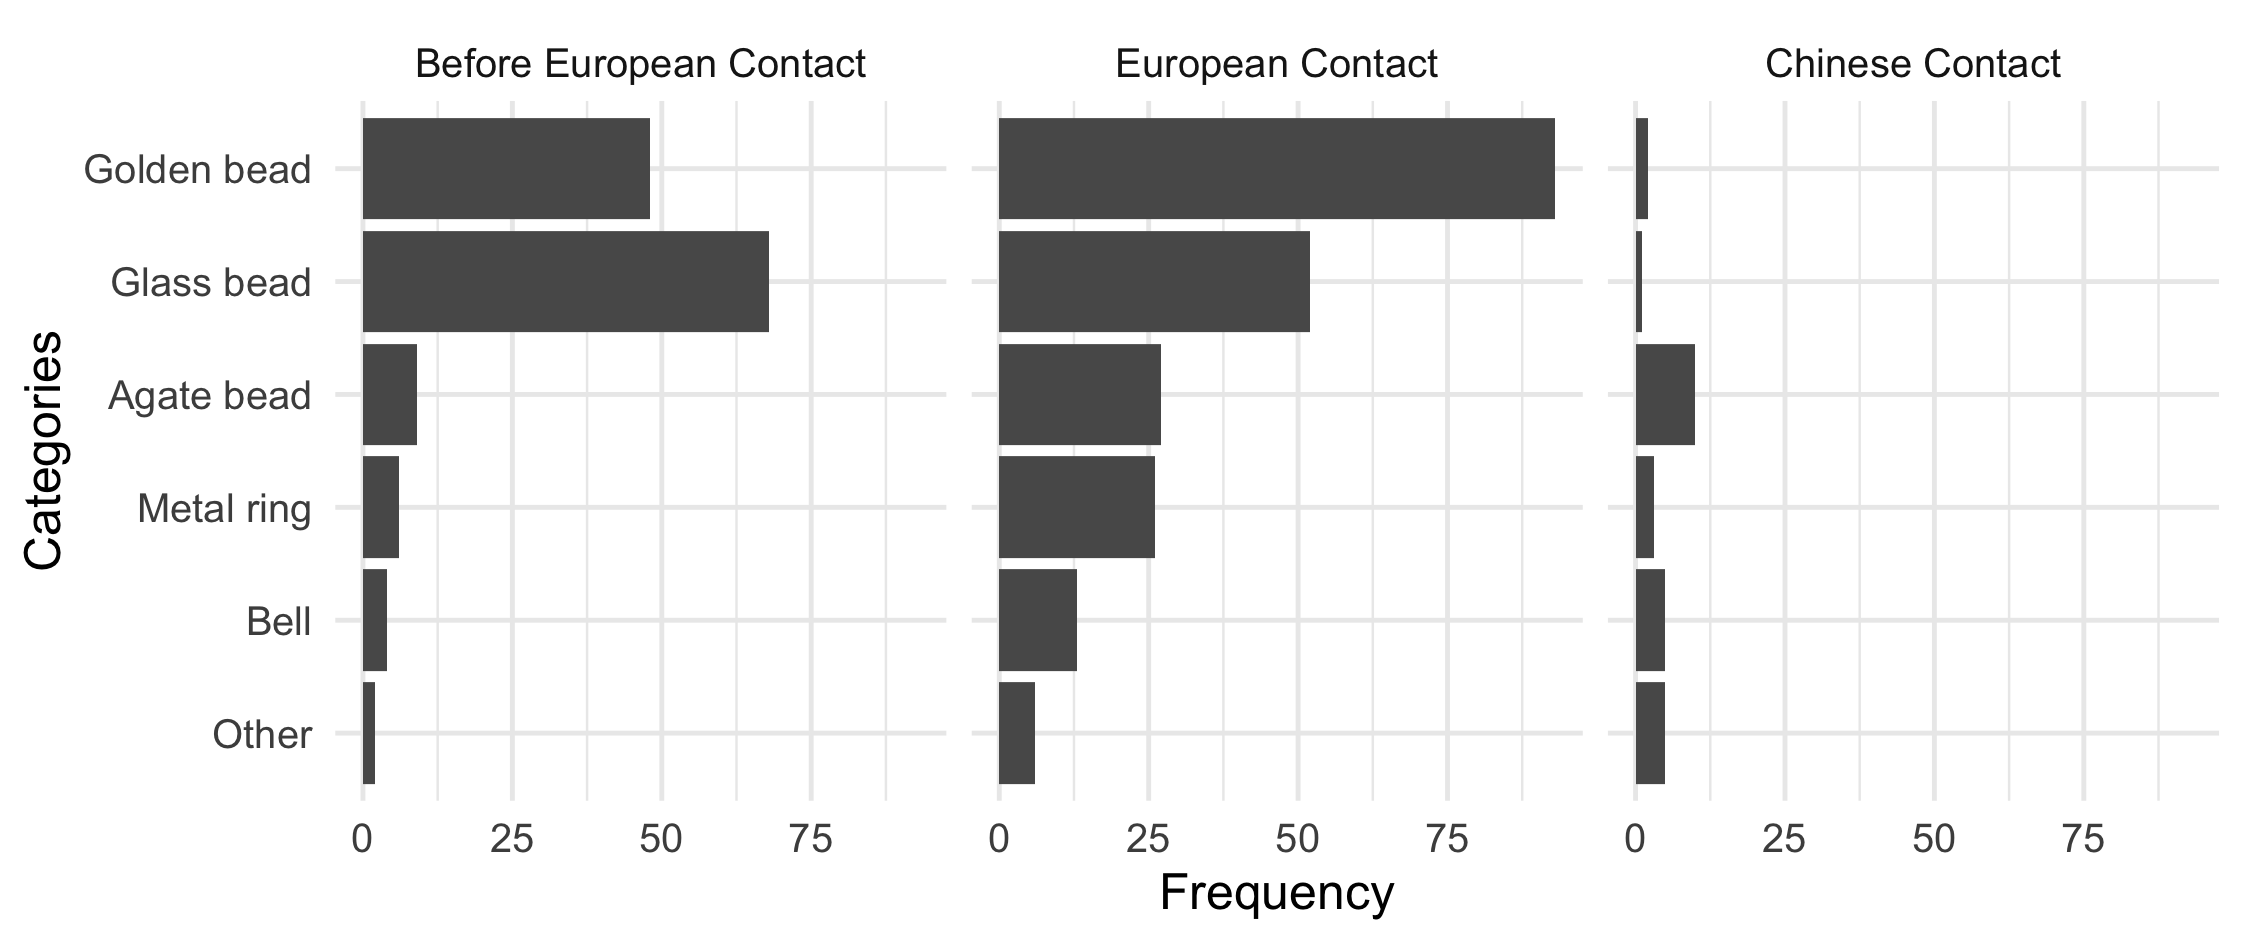
\includegraphics[width=5.31in]{/Users/bmarwick/Desktop/kwl-ornaments/analysis/figures/plot-ornaments-count-three-periods} \caption{Frequency of the major ornament across different time periods.}(\#fig:plot-counts-by-period)
\end{figure}

\hypertarget{results}{%
\section{Results}\label{results}}

\hypertarget{changes-in-the-frequencies-of-ornament-types-over-time}{%
\subsection{Changes in the frequencies of ornament types over
time}\label{changes-in-the-frequencies-of-ornament-types-over-time}}

Figure @ref(fig:plot-counts-by-period) shows the comparison of
frequencies of the major classes of ornaments for different the time
periods at Kiwulan. The difference in frequencies between the three time
periods reflect significant differences in the use of ornaments
(chi-square = 71.82, df = 8, p-value =
\(\ensuremath{2.136325\times 10^{-12}}\)). Most ornament types were
present before European contact. Ornament frequencies reached a peak
during the European period and then dropped during the Chinese period,
especially gold-foil beads. This trend can be also seen on other
ornaments including carnelian beads, metal rings, and bells. However,
glass beads show a different pattern that indicates a higher frequency
in the pre-European contact, and then a decrease in the European period
and a further decrease in the Chinese period.

\begin{figure}
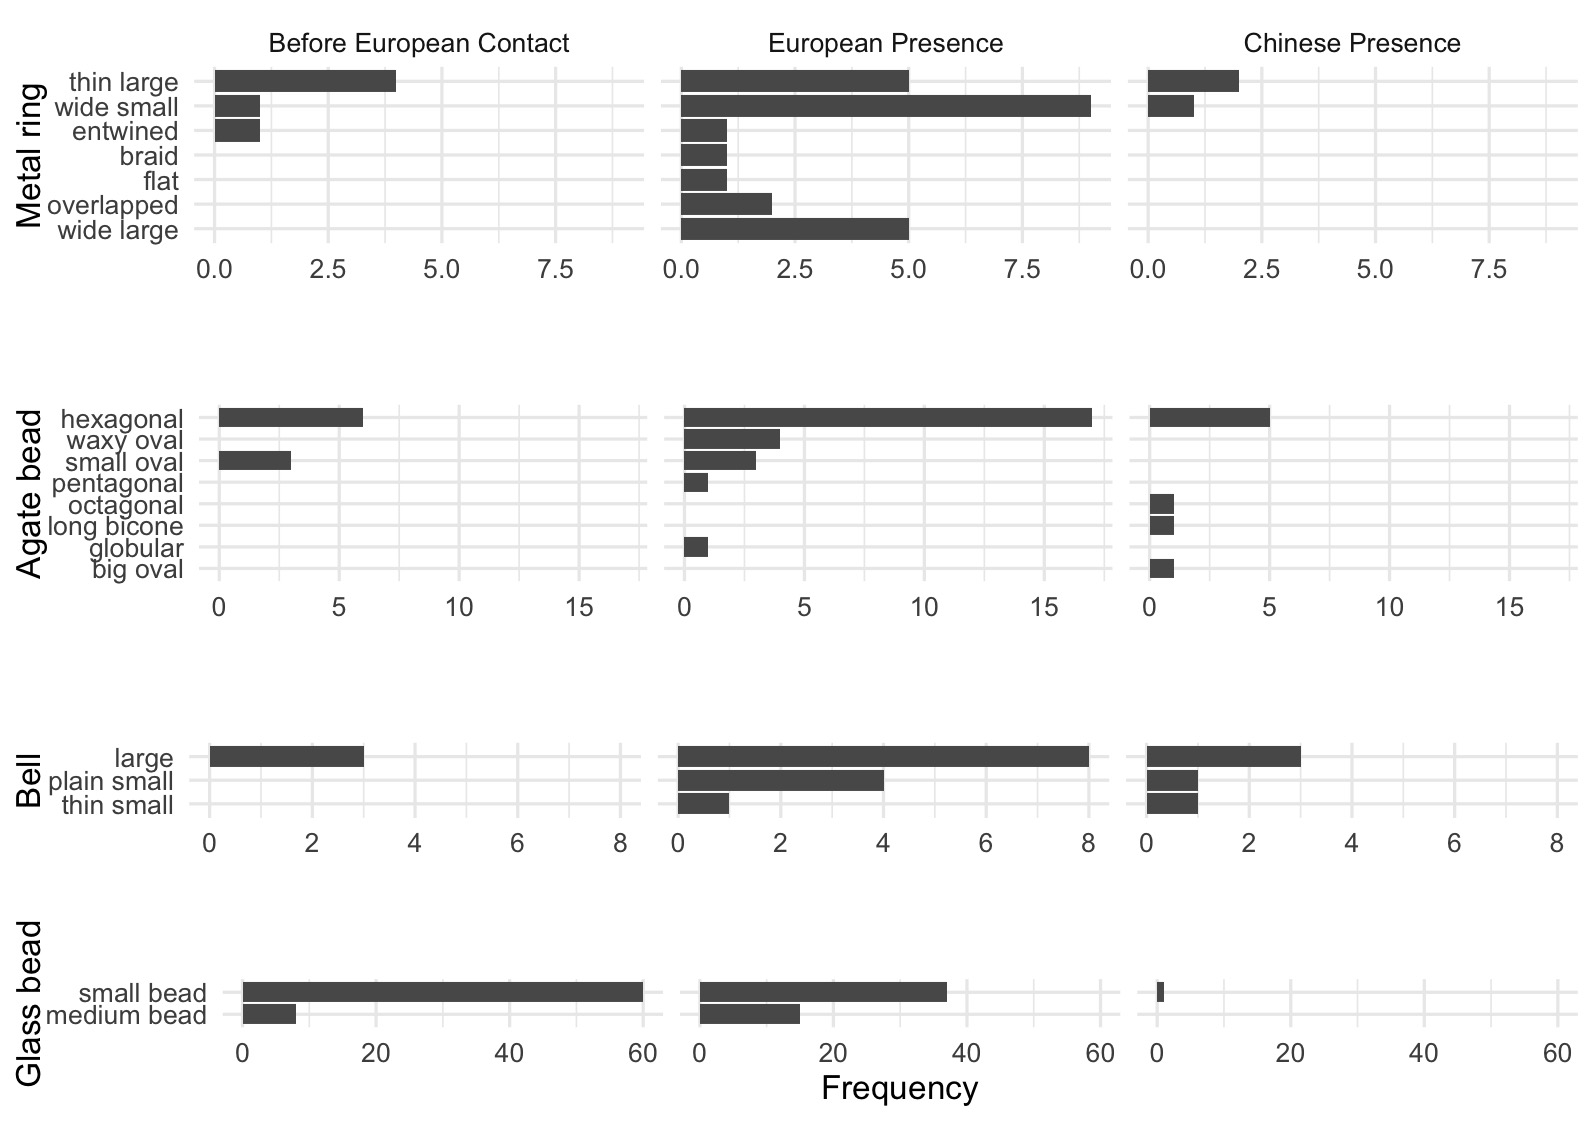
\includegraphics[width=5.31in]{/Users/bmarwick/Desktop/kwl-ornaments/analysis/figures/plot-multi-types-by-period} \caption{Frequency of ornament subtypes showing the changes in frequency across time periods for metal rings, carnelian beads, bells, and glass beads.}(\#fig:plot-altogether)
\end{figure}

The distribution of frequencies for subtypes in each major class is
presented in Figure @ref(fig:plot-altogether). Spearman's correlation
test shows that there is no significant relationship between diversity
of subtypes and sample size (S = 498.09, rho = 0.11, p = \(0.69489\)).
This indicates that the increases in diversity can be explained by the
effects of culture interaction instead of the effects of sample size.
Carnelian beads and metal rings have greater quantity and variety of
shapes compared to copper bells and glass beads during the European
period. The greater varieties for carnelian beads and metal rings might
indicate multiple origins due to participation in large scale trade
networks stimulated by the European presence. In contrast, copper bells
have less variety typically \textgreater2 cm long with a wide variety of
human faces as a motif. Although glass beads have less variety in size,
small (0.5-1 cm) and medium (1-2 cm), they have a wide variety of colors
or patterns mostly made by winding technique with high lead content in
composition indicating possibly from China (Cheng 2008). Although we are
not certain of the specific origin of these beads, research suggest that
these glass beads and metal ornaments have similar production techniques
and composition to those found in China (Chen 2011; Wang 2018). There
seem to be no obvious changes in the sources of glass beads or metal
ornaments at different periods in the upper component of Kiwulan
(1400-1900 AD). However, the glass beads found from the lower component
(700-1200 AD) are mostly Indo-Pacific beads, widespread in Southeast
Asian sites since 300 BC and declining during the early 2nd millennium
(Wang 2018; Francis 2002).

\begin{figure}
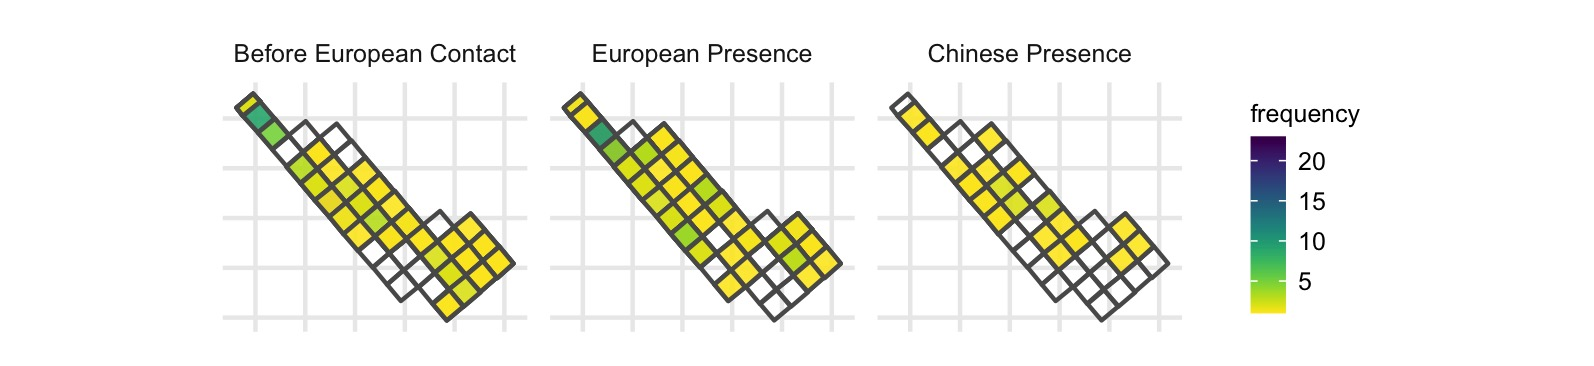
\includegraphics[width=5.31in]{/Users/bmarwick/Desktop/kwl-ornaments/analysis/figures/plot-spatial-distribution-all-ornaments-by-period} \caption{Spatial pattern of all class of ornament by time periods}(\#fig:plot-all-spatial-pattern)
\end{figure}

\begin{figure}
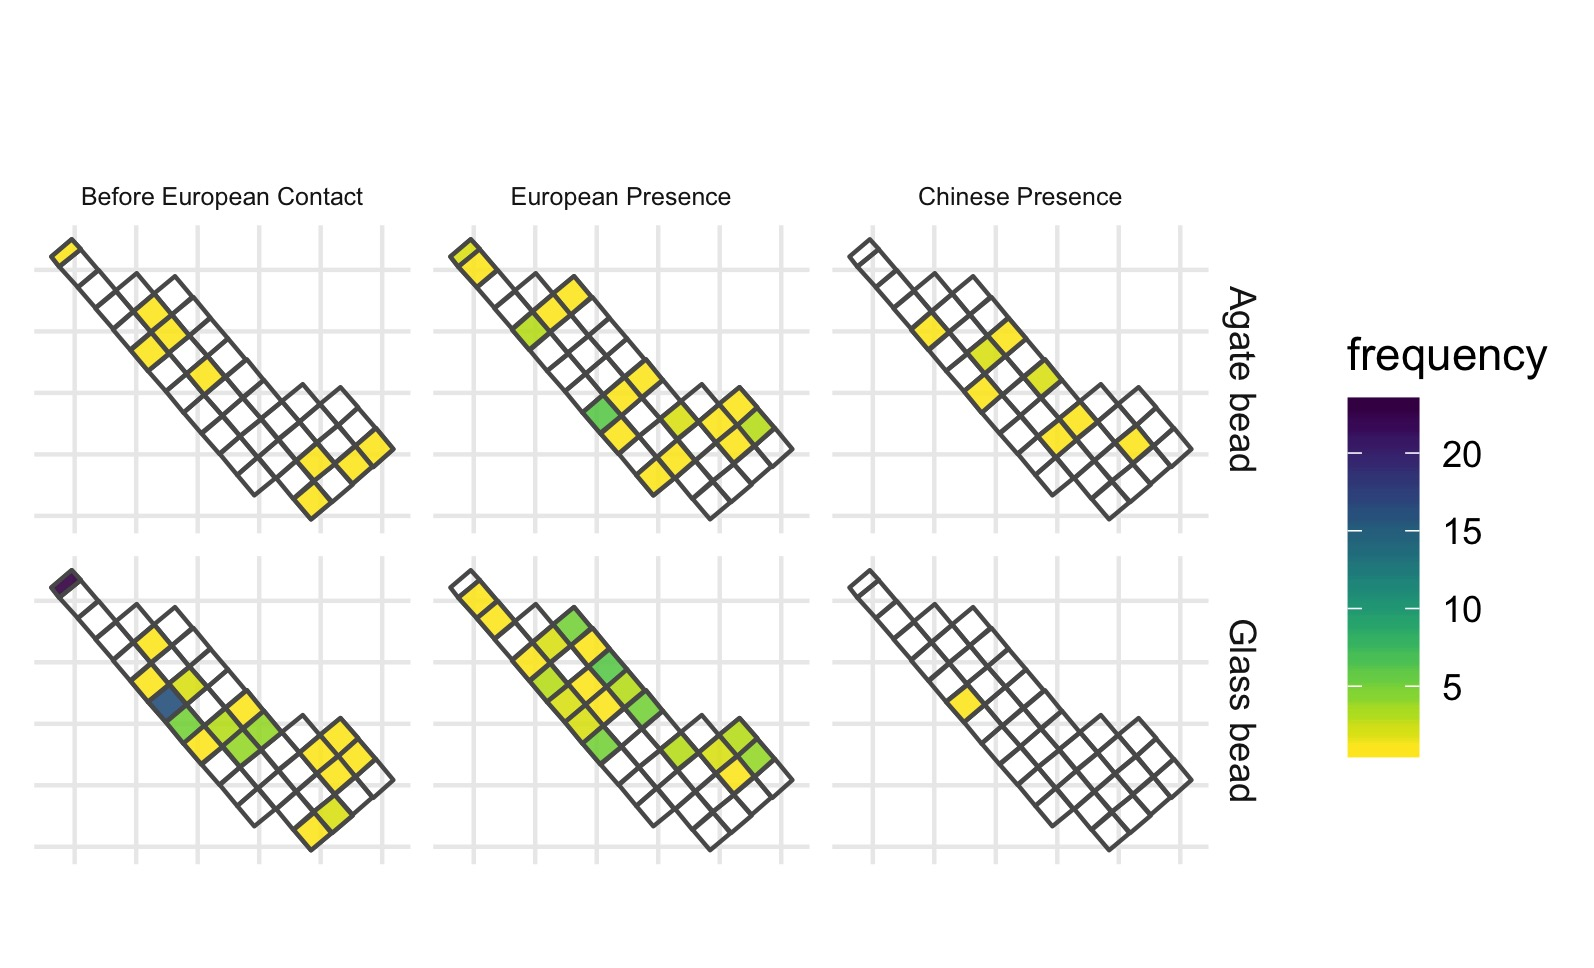
\includegraphics[width=5.31in]{/Users/bmarwick/Desktop/kwl-ornaments/analysis/figures/plot-spatial-distribution-some-ornaments-by-period} \caption{Spatial pattern for ornament class by time periods, only those types with more than 5 pieces are shown here}(\#fig:plot-spatial-pattern-each)
\end{figure}

\hypertarget{changes-in-patterns-of-the-spatial-distribution-of-ornament-types}{%
\subsection{Changes in patterns of the spatial distribution of ornament
types}\label{changes-in-patterns-of-the-spatial-distribution-of-ornament-types}}

Figure @ref(fig:plot-all-spatial-pattern) presents the spatial
distribution of all ornaments from the research area for each time
period. Before the European arrival, a greater amount of ornaments were
found at the northern and middle parts of the research area. During the
European period, ornaments were more widespread, with some clusters on
the northern part. During the Chinese period the distribution is more
even again. Figure @ref(fig:plot-spatial-pattern-each) presents the
distribution for the major ornament classes individually, some clusters
across the area can be observed during the European period, such as
gold-foil beads and carnelian beads. However, there seems to be no
consistent pattern across those different ornaments. Each class shows
its own pattern where the squares with higher numbers of ornaments
distributed separately and independently. For example, a cluster of
gold-foil beads was found at the northern part, while a cluster of
carnelian beads was found in the middle part. In contrast, there are
multiple clusters of metal rings that are distributed separately across
the research area. Copper bells were usually found individually and
appear randomly distributed across the area. In the Chinese period, both
the amount and density of different classes of ornaments decreased.

\begin{figure}
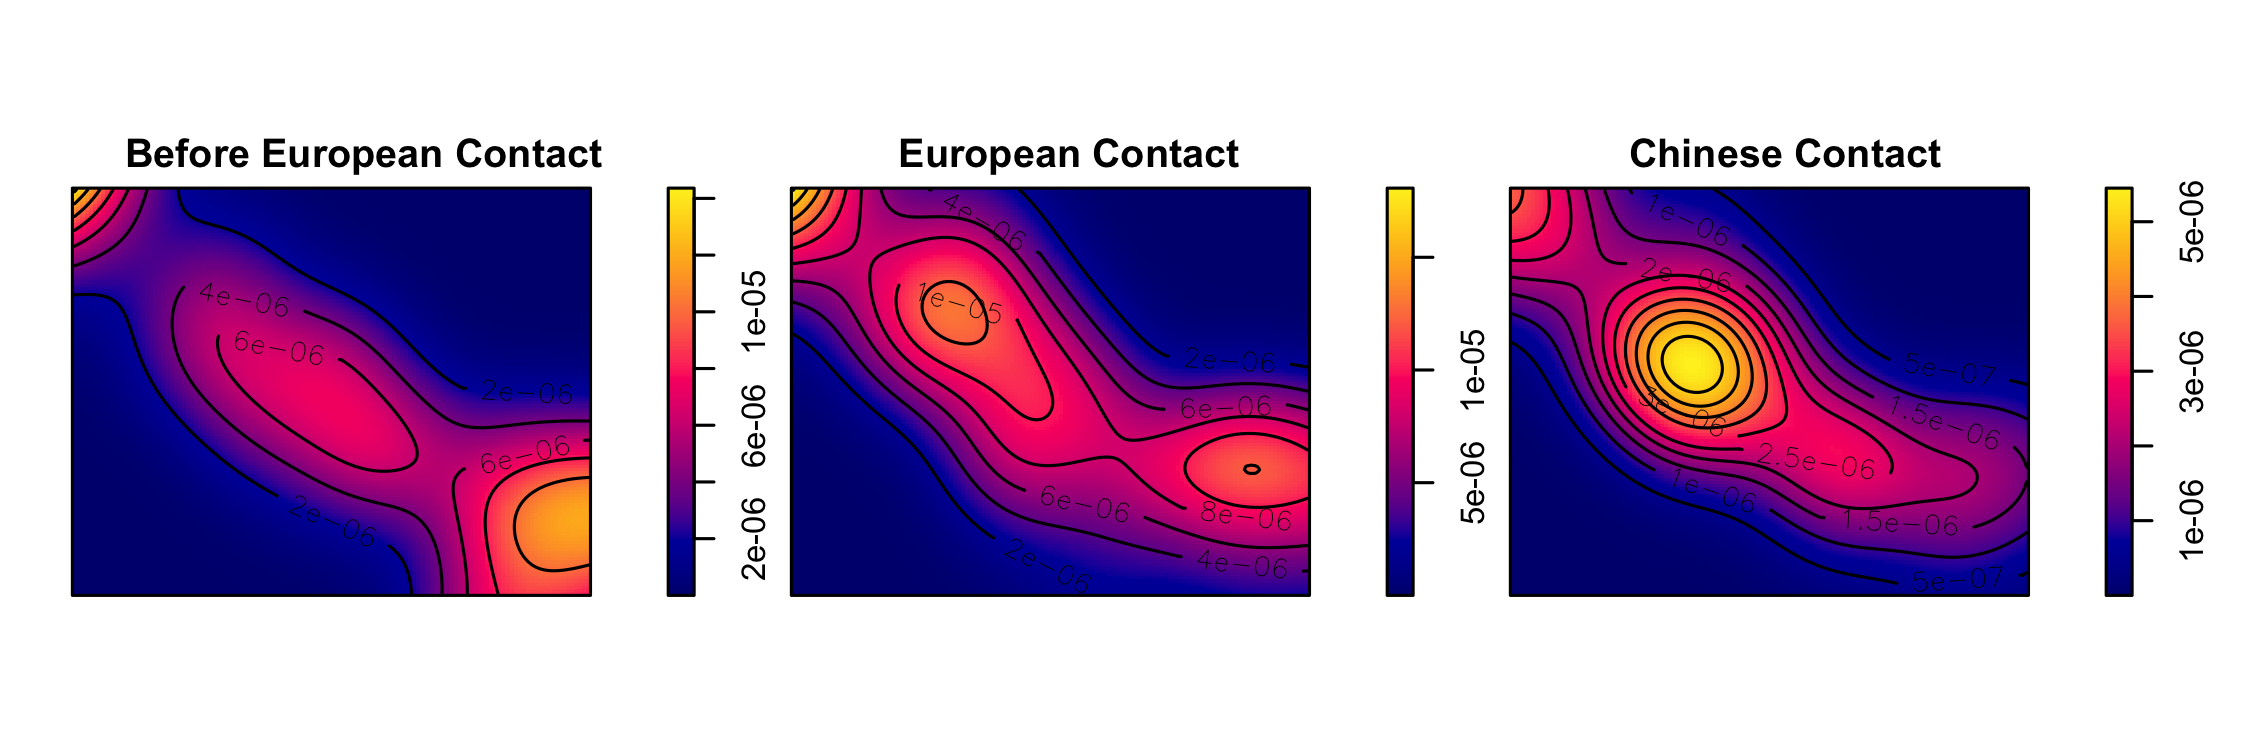
\includegraphics[width=5.31in]{/Users/bmarwick/Desktop/kwl-ornaments/analysis/figures/plot-kde-maps} \caption{Kernel density map for ornaments by periods. Used the bandwidth based on Silverman (1986)'s rule of thumb.}(\#fig:plot-all-densities)
\end{figure}

\hypertarget{point-pattern-analysis-of-ornament-distribution}{%
\subsection{Point pattern analysis of ornament
distribution}\label{point-pattern-analysis-of-ornament-distribution}}

Point pattern analysis can assess whether the distribution of artefacts
represents hotspots produced by non-random processes (Bevan \& Lake
2016; Ducke 2015), such as concentrations of ornaments in specific
households that might result from social inequality stimulated by a
colonial presence. To prepare the ornament location data for point
pattern analysis, because artefacts from Kiwulan lack exact
piece-provance data, we assigned each ornament to a random coordinate
pair in the square it was recovered from. The next step was to divide
the ornaments into three time periods. Finally we computed the kernel
densities for each time period for comparison. Kernel density
estimations (KDE) compute the probability of the density of ornaments
across space by creating a continuous, smooth density surface across
space. Here we use KDE to visualize core areas of ornaments and
surrounding neighbourhoods (Bonnier \emph{et al.} 2019; Cortegoso
\emph{et al.} 2016). Density values of artefacts per square meter were
calculated for each cell.

Figure @ref(fig:plot-all-densities) shows that there is one major core
area during the pre-European period, multiple core areas during the
European period, and a single core during the Chinese period. There are
three consistent sub-regions with a core area that shifts over time. The
distribution might indicate the increase and decrease in the number of
social groups who possessed ornaments. The multiple groups during the
European period might reflect unequal consumption of ornaments across
the site, relative to other periods, or random patterns resulting from a
bigger sample size. In addition, the generation of core areas might be
biased due to small sample sizes, for example, a few ornaments found at
one single square during the Chinese period could create an obvious
hotspot. Whether the observed clustering is random or non-random is
crucial for the interpretation of intentional human activities.

\begin{figure}
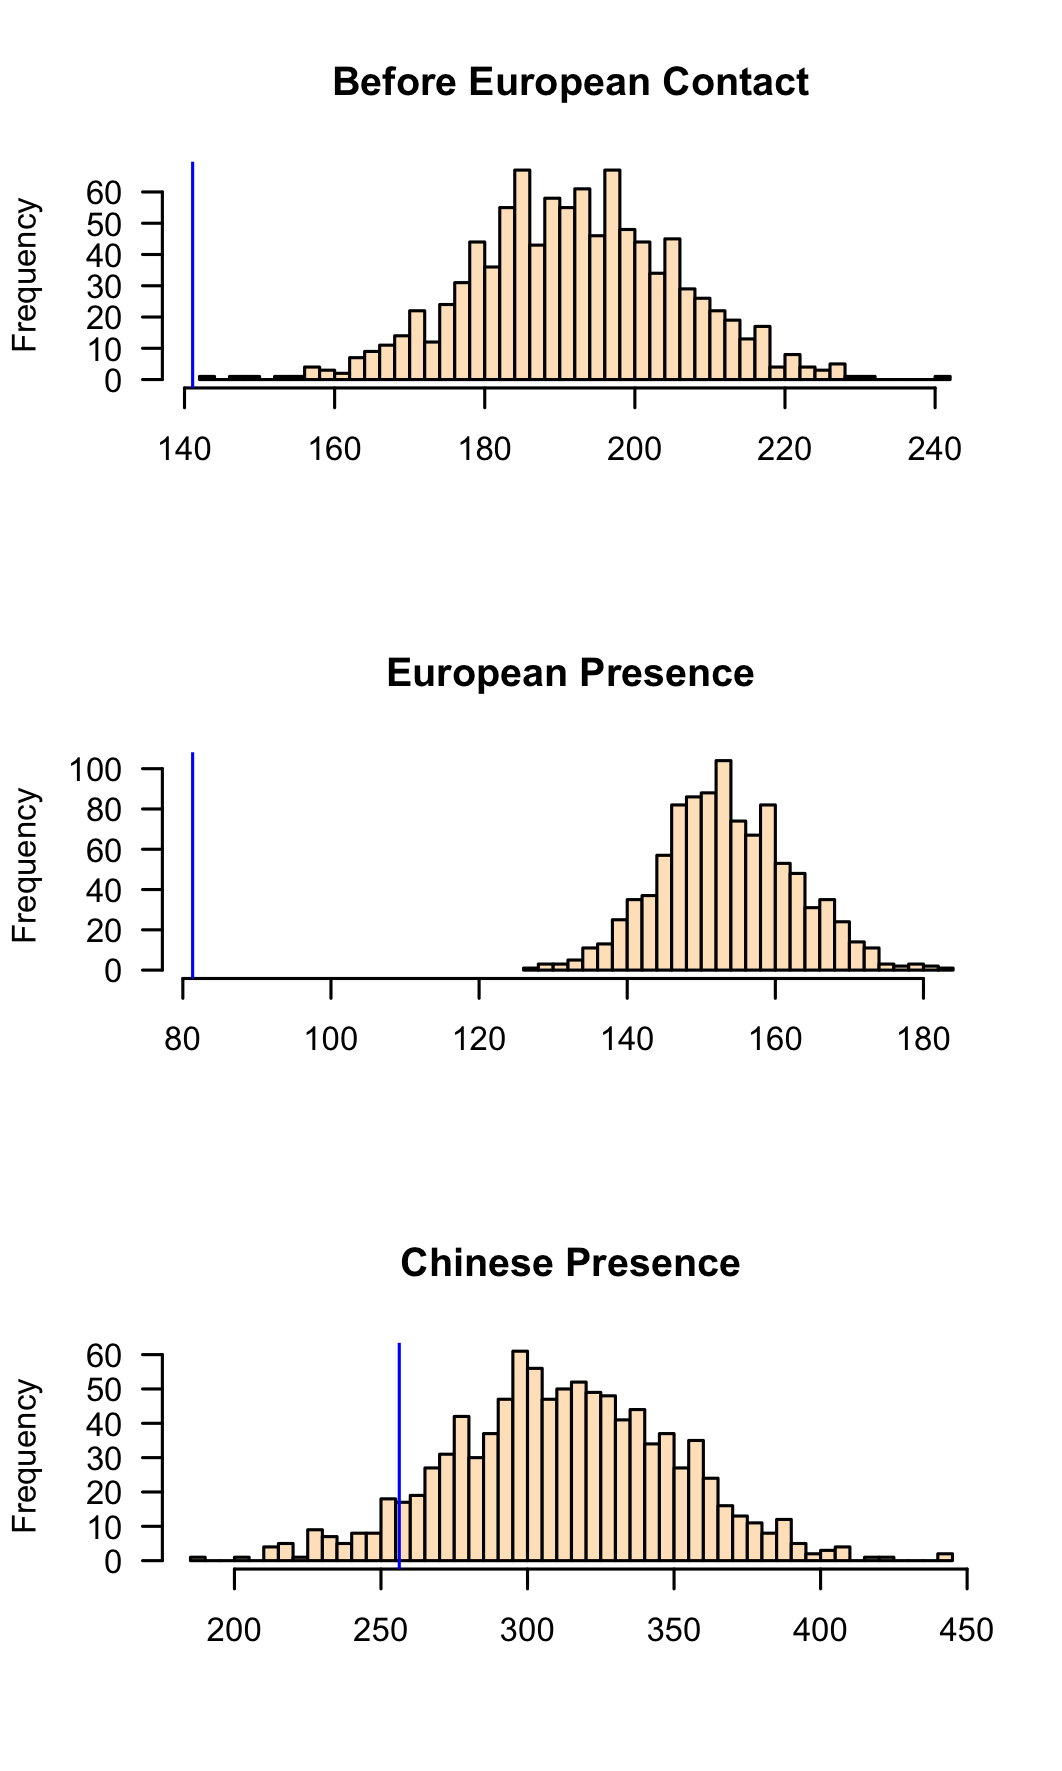
\includegraphics[width=3.54in]{/Users/bmarwick/Desktop/kwl-ornaments/analysis/figures/plot-kde-ann-histograms} \caption{Histograms of simulated ANN values from 1000 simulations for three time periods. X-axis values represent ANN expected value under a completely random process resulted from simulated pattern. Each sample distribution presents the null hypothesis with the blue line indicating the observed ANN value.}(\#fig:hypo-test-distribution)
\end{figure}

To test for randomness in spatial locations, we used a Monte Carlo
method to simulate average nearest-neighbour distances (ANN). Figure
@ref(fig:hypo-test-distribution) shows the observed ANN distances with
the distributions of the ANN distances calculated on 1000 simulations of
random ornament locations. The results show that 100\% of the simulated
values are much greater than our observed ANN value during the European
period, which means the ornaments have non-randomly clustered
distributions. A similar, but less extreme, result is also observed
during the pre-European period. The observed distribution of ornaments
is more similar to the random distributions during the Chinese period,
with about one third of the simulated values are greater than our
observed ANN value. The Chinese period has fewer artefacts in any
category, likely reflecting a smaller population at Kiwulan at this
time, making spatial patterns and hotspots difficult to discern with
confidence. This testing reveals clustering of ornaments during the
European period is highly non-random, potentially indicating different
degrees of access to foreign ornaments or a concentration of power to
control the distribution of ornaments at Kiwulan during this period.

\hypertarget{discussion}{%
\section{Discussion}\label{discussion}}

An indirect colonial influence may be indicated at Kiwulan by the
greater diversity of ornament types and materials during the European
period. Yilan was involved in complex trading networks both on a
regional scale with other indigenous groups and Chinese merchants, and
at a global scale with Europeans, including the Dutch and the Spanish.
The ornaments have multiple origins, including Southeast Asia and China,
and were first introduced into northeastern Taiwan by Chinese merchants
before 17th century. Later, trade activities became more frequent and
intense in the 17th century due to European activities. The greater
diversity and quantity of ornaments likely results from participation in
large scale exchange networks that stimulated the circulation of
different ornament classes. The frequency of overall ornaments and each
subtype declines significantly after European influence fades during the
Chinese period in the early 19th century. This may be due to a smaller
scale of trading networks, the overall decline of indigenous populations
in Yilan, or the adoption of Han Chinese practices. The decline of the
population may be related to the movement of many indigenous people
moved southwards to Hualien due to population pressure caused by Han
Chinese immigrants at the end of the 18th century (Chen 2007).

Archaeological contexts show that ornaments are especially abundant in
burial contexts serving as grave goods. This supports the interpretation
of ornaments as valuable objects functioning as status indicators.
Spatial patterns of ornaments in dwelling contexts show that their
distribution was clustered during the pre-European and European periods.
These clusters are non-random, and are most highly concentrated during
the European period. This may indicate that a degree of social
inequality based on the uneven distribution of ornaments was already
present before European contact, and then it was reinforced and
amplified during the European period. A further indicator of increased
social inequality is a burial dated to the 17th century that included 60
gold-foil beads, well above the average of 2-3 pieces in the
pre-European period (Chen 2007; Cheng 2008).

How might these results fit into a bigger picture of social change at
periphery of colonial systems? We may get some insight into the general
pathways that led to social inequality in northeastern Taiwan by
considering how people have achieved and maintained power in a wide
variety of societies (Drennan \emph{et al.} 2010; Feinman 2000; Ames
2010; Bowles \emph{et al.} 2010). The corporate/network model proposed
by Feinman (2000) expands traditional hierarchical complexity to provide
a comparative basis for distinct strategies for power. In the network
mode, inequality develops when individuals accumulate wealth through
their individual networks and people use their wealth to attract
factions, control resources, and monopolize trade networks. In contrast,
the corporate mode stresses shared power across different groups and
sectors, integrative ceremonies and rituals, and large cooperative
labour tasks (Feinman 2000; Siegel 1999). We may be able to interpreate
Yilan social organisation as moving from corporate mode before the
European arrival, to a network mode during European presence. The small
number of ornaments, and less concentrated distribution during the
pre-European period appears consistent with shared power and wealth of
the corporate mode. The long-distance trade network introduced by
Europeans resulted in the appearance of a network mode, and the
emergence of competition among ambitious individuals for prestige,
wealth, or power through collecting trade goods (Brumfiel 1994; Clark \&
Blake 1994). Because of the weak direct control from the European
colonizers in northeastern Taiwan, local leaders may have had the
flexibility to manipulate European colonial images, expand personal
power, and monopolize the high-value trade goods (Kang 2012).

That said, the evidence from Kiwulan may be consistent with a variety of
scenarios of indigenous-colonial relations. The increasing number and
concentrated spatial patterns of ornaments may indicate a practice of
cultural resistance against the European intrusion. Resistance to
European economic and political demands may be inferred if ornaments
were used as a display of social identity and to emphasize the local
customs that had existed before European contact (cf.~Rubertone 2000).
Resistance could be presented in many forms. Another scenario is that
ornaments were treated as heirlooms, such as carnelian beads and
gold-foil beads, that passed from one generation to the next,
accumulating at Kiwulan over time. This process would result in a
natural increase in ornaments over time, unrelated to colonial
influences, but has limited value in explaining the shifts in spatial
patterns.

\hypertarget{conclusion}{%
\section{Conclusion}\label{conclusion}}

Examination of the archaeological record at the peripheries of colonial
activities can show how remote indeignous groups were affected by major
European colonial processes (Trabert 2017). Kiwulan in northeastern
Taiwan is an exceptional case study as an East Asian location that was
relatively isolated and peripheral, and yet connected by regional and
global trade networks. Kiwulan provides valuable insights into the
discussion of indirect colonial influence on local societies living
beyond the borders of direct European colonial occupation. The frequency
and spatial distribution of personal ornaments at Kiwulan present three
distinct patterns during different dominant culture interaction periods.
The greater amount and diversity of ornament types during the European
period reflects an increasing use in ornaments in a colonial context.
Before European contact, ornaments were traded into local indigenous
societies via the regional exchagne network with Chinese merchants and
viewed as prestige goods in local indigenous culture according to their
distribution in the archaeological contexts. After the arrival of the
Europeans, the exotic and powerful image carried by those ornaments may
have intensified, further signalling wealth and privileged trading
connections among the inhabitants of Kiwulan. This may have stimulated
more competition between aggrandizing individuals for prestige and
wealth accumulation at Kiwulan, which might have resulted in an increase
in social inequality. This might also indicate an act of intentional
resistance to the intrusion of the Europeans by using more ornaments
that is part of culture tradition.

We are still far from understanding the full variety of colonial impacts
on peripheral indigenous communities. The origin of ornaments and how
their sources changed over time would give more information to construct
a clear picture of complex trade networks during this periods. By
focusing on the distribution patterns in a settlement site, the Kiwulan
ornaments suggest that foreign ornaments can be a proxy to detect
indirect colonial influence on local indigenous populations. Ornaments
give insights into the amplification of social inequality stimulated by
European colonisation. It also shows the agency of indigenous people to
incorporate ornaments into their social system and use them in their
daily lives to display or intensify status differences. Future work
could extend this approach to sourcing the ornaments directly with
geochemical methods, and studies of other trade goods such as ceramics.
We have introduced here the corporate/network model for understanding
the dynamics of social inequality at Kiwulan, and future tests of this
should include analysis of pottery production and standardisation, and
mortuary practices.

\hypertarget{acknowledgements}{%
\section{Acknowledgements}\label{acknowledgements}}

We would like to thank the Yilan County Cultural Affairs Bureau in
Taiwan for permitting access to the ornaments used in this study. We
thank Shui-jin Chiu, Shu-hui Jian, Jiun-yao Lai, and the staff in
archaeology lab for their invaluable assistance in preparing samples for
analysis. We also thank Yu-pei Chen for the discussion regarding the
site at the earliest stage of fieldwork. This work was supported in part
by the Fritz Graduate Fellowship and travel grants from the Department
of Anthropology at University of Washington. We would also like to thank
Ben Fitzhugh and Peter Lape for their insightful comments on the early
draft.

\hypertarget{pagebreak}{%
\subparagraph{pagebreak}\label{pagebreak}}

\hypertarget{references}{%
\section{References}\label{references}}

\hypertarget{refs}{}
\leavevmode\hypertarget{ref-Ames2010}{}%
\textsc{Ames}, K.M. 2010. On the evolution of the human capacity for
inequality and/or egalitarianism, in G. Feinman \& T.D. Price (ed.)
\emph{Pathways to power: New perspectives on the emergence of social
inequality}: 15--44. New York: Springer.

\leavevmode\hypertarget{ref-Andrade2007}{}%
\textsc{Andrade}, T. 2007. \emph{How Taiwan became chinese : Dutch,
spanish, and han colonization in the seventeenth century}. New York:
Columbia University Press.

\leavevmode\hypertarget{ref-Bellina2014}{}%
\textsc{Bellina}, B. 2014. Maritime silk roads' ornament industries:
Socio-political practices and cultural transfers in the south china sea
\emph{Cambridge Archaeological Journal} 24. Cambridge University Press:
345--77.

\leavevmode\hypertarget{ref-Berrocal2018}{}%
\textsc{Berrocal}, M.C., E.S. \textsc{Herrero}., M.G. \textsc{Moret}.,
A.U. \textsc{González}., M.T. \textsc{Pérez}., S.C. \textsc{Rodrı́guez}.,
A. \textsc{Chevalier}., F. \textsc{Valentin}. \& C.-h. \textsc{Tsang}.
2018. A comprised archaeological history of taiwan through the long-term
record of heping dao, keelung \emph{International Journal of Historical
Archaeology} 22. Springer: 905--40.

\leavevmode\hypertarget{ref-Bevan2016}{}%
\textsc{Bevan}, A. \& M. \textsc{Lake}. 2016. Intensities, interactions,
and uncertainties: Some new approaches to archaeological distributions,
in A. Bevan \& M. Lake (ed.) \emph{Computational approaches to
archaeological spaces}: 27--52. Routledge.

\leavevmode\hypertarget{ref-Blusse2000}{}%
\textsc{Blussé}, L. \& N. \textsc{Everts}. 2000. \emph{(FEII) the
formosan encounter. Notes on formosa's aboriginal society, a selection
of documents from dutch archival sources. Volume ii: 1636-1645}. Taipei:
Shung Ye Museum of Formosan Aborigines, Taipei.

\leavevmode\hypertarget{ref-Bonnier2019}{}%
\textsc{Bonnier}, A., M. \textsc{Finné}. \& E. \textsc{Weiberg}. 2019.
Examining land-use through gis-based kernel density estimation: A
re-evaluation of legacy data from the berbati-limnes survey
\emph{Journal of Field Archaeology} 44. Taylor \& Francis: 70--83.

\leavevmode\hypertarget{ref-Borao2001}{}%
\textsc{Borao}, H., J. E. 2001. \emph{(SIT, pp. 1-343). Spaniards in
taiwan, vol. I (1582--1641)}. Taipei: SMC Publishing.

\leavevmode\hypertarget{ref-Borao2009}{}%
\textsc{Borao}, J.E. 2009. \emph{The spanish experience in Taiwan,
1626-1642: The baroque ending of a renaissance endeavor}. Hong Kong:
Hong Kong University Press.

\leavevmode\hypertarget{ref-Bowles2010}{}%
\textsc{Bowles}, S., E. \textsc{Smith}. \& M. \textsc{Mulder}. 2010. The
emergence and persistence of inequality in premodern societies
\emph{Current anthropology} 51: 7--17.

\leavevmode\hypertarget{ref-Brumfiel1994}{}%
\textsc{Brumfiel}, E.M. 1994. Factional competition and political
development in the new world: An introduction, in E.M. Brumfiel \& J.
Fox (ed.) \emph{Factional competition and political development in the
new world}: 3--13. Cambridge: Cambridge University Press.

\leavevmode\hypertarget{ref-Carter2016}{}%
\textsc{Carter}, A.K. 2016. The production and exchange of glass and
stone beads in southeast asia from 500 bce to the early second
millennium ce: An assessment of the work of peter francis in light of
recent research \emph{Archaeological Research in Asia} 6. Elsevier:
16--29.

\leavevmode\hypertarget{ref-Chen2011}{}%
\textsc{Chen}, K.-t. 2011. A preliminary research of copper-based
artifacts and related remains discovered in the taiwan area \emph{Chung
Yang Yen Chiu Yuan Li Shih Yu Yen Yen Chiu So Chi K'an {[}Bulletin of
the Institute of History and Philology Academia Sinica{]}} 82: 169--259.

\leavevmode\hypertarget{ref-Chen1963}{}%
\textsc{Chen}, S. 1963. \emph{Kavalan ting zhi {[}kavalen culture
history{]}, taiwan wen xian cong kan di 106 zhong {[}taiwan literature
series: 106{]}}. Taipei: Economic Research Office, Bank ofTaiwan.

\leavevmode\hypertarget{ref-Chen2005}{}%
\textsc{Chen}, T.-j. 2005. \emph{Ji long shan yu dan shui yang : Dong ya
hai yu yu tai wan zao qi yan jiu, 1400-1700 {[}mount keelung and tai she
ocean: A study of east asian seas and the hisotry of Taiwan from 1400 to
1700{]}.} Taipei: Lian jing.

\leavevmode\hypertarget{ref-Chen2017}{}%
\textsc{Chen}, W.-c. 2017. The early occupation of taiwan, in J. Habu,
P.V. Lape, \& J.W. Olsen (ed.) \emph{Handbook of east and southeast
asian archaeology}: 277--91. Springer.

\leavevmode\hypertarget{ref-Chen2007}{}%
\textsc{Chen}, Y.-p. 2007. \emph{Qi wu lan yi zhi qiang jiu fa jue bao
gao {[}report on the archaeological excavations at ki-wu-lan site{]}}.
Yilan, Taiwan: Lanyang museum.

\leavevmode\hypertarget{ref-Cheng2008}{}%
\textsc{Cheng}, C.-F. 2008. Qi wu lan yi zhi yu she nei yi zhi chu tu bo
li zhu de xiang guan yan jiu {[}studies of glass beads excavated from
kivulan and shenei site, taiwan{]}. Master's thesis.

\leavevmode\hypertarget{ref-Chiu2004}{}%
\textsc{Chiu}, H.-L. 2004. Yilan xian jiao xi xiang qi wu lan yi zhi chu
tu mu zang yan jiu ──mai zang hang wei yu wen hua bian qian de guan cha
{[}investigations of mortuary behaviors and cultural change of the
kivulan site in i-lan county{]}. Master's thesis.

\leavevmode\hypertarget{ref-Clark1994}{}%
\textsc{Clark}, J.E. \& M. \textsc{Blake}. 1994. The power of prestige:
Competitive generosity and the emergence of rank societies in lowland
mesoamerica \emph{Factional competition and political development in the
New World}, 17--30.

\leavevmode\hypertarget{ref-Cort2017}{}%
\textsc{Cort}, L.A. 2017. Container jars from the maenam noi kilns,
thailand use and reuse along maritime trade routes in asia
\emph{Bulletin de l'École française d'Extrême-Orient} 103. École
française d'Extrême-Orient: 267--96.

\leavevmode\hypertarget{ref-Cortegoso2016}{}%
\textsc{Cortegoso}, V., R. \textsc{Barberena}., V. \textsc{Durán}. \& G.
\textsc{Lucero}. 2016. Geographic vectors of human mobility in the andes
(34--36° s): Comparative analysis of `minor'obsidian sources
\emph{Quaternary International} 422. Elsevier: 81--92.

\leavevmode\hypertarget{ref-Dietler1997}{}%
\textsc{Dietler}, M. 1997. The iron age in mediterranean france:
Colonial encounters, entanglements, and transformations \emph{Journal of
World Prehistory} 11. Springer: 269--358.

\leavevmode\hypertarget{ref-Dietler2005}{}%
--- 2005. The archaeology of colonization and the colonization of
archaeology: Theoretical challenges from an ancient mediterranean
colonial encounter, in G. Stein (ed.) \emph{The archaeology of colonial
encounters: Comparative perspectives}: 33--68. Santa Fe: NM: Sch. Am.
Res. Press.

\leavevmode\hypertarget{ref-Dietler2015}{}%
--- 2015. \emph{Archaeologies of colonialism: Consumption, entanglement,
and violence in ancient mediterranean france}. Univ of California Press.

\leavevmode\hypertarget{ref-Drennan2010}{}%
\textsc{Drennan}, R.D., C.E. \textsc{Peterson}. \& J.R. \textsc{Fox}.
2010. Degrees and kinds of inequality, in \emph{Pathways to power}:
45--76. Springer.

\leavevmode\hypertarget{ref-Ducke2015}{}%
\textsc{Ducke}, B. 2015. Spatial cluster detection in archaeology:
Current theory and practice, in J.A. Barcelo \& I. Bogdanovic (ed.)
\emph{Mathematics and archaeology}: 352--68. Barcelona, Spain: CRC Press
Boca Raton.

\leavevmode\hypertarget{ref-Feinman2000}{}%
\textsc{Feinman}, G.M. 2000. Corporate/network: New perspectives on
models of political action and the puebloan southwest \emph{Social
Theory in Archaeology, University of Utah Press, Salt Lake City},
31--51.

\leavevmode\hypertarget{ref-Francis2002}{}%
\textsc{Francis}, P. 2002. \emph{Asia's maritime bead trade: 300 bc to
the present}. University of Hawaii Press.

\leavevmode\hypertarget{ref-Galloway2006}{}%
\textsc{Galloway}, P. 2006. Material culture and text: Exploring the
spaces within and between \emph{Historical archaeology} 9. Blackwell
Publishing.

\leavevmode\hypertarget{ref-Gan2006}{}%
\textsc{Gan}, F., H. \textsc{Cheng}. \& Q. \textsc{Li}. 2006. Origin of
chinese ancient glasses---study on the earliest chinese ancient glasses
\emph{Science in China Series E: Technological Sciences} 49. Springer:
701--13.

\leavevmode\hypertarget{ref-Given2004}{}%
\textsc{Given}, M. 2004. \emph{The archaeology of the colonized}.
London; New York: Routledge.

\leavevmode\hypertarget{ref-Grave2013}{}%
\textsc{Grave}, P. \& I.J. \textsc{McNiven}. 2013. Geochemical
provenience of 16th--19th century ce asian ceramics from torres strait,
northeast australia \emph{Journal of Archaeological Science} 40.
Elsevier: 4538--51.

\leavevmode\hypertarget{ref-Hsieh2009}{}%
\textsc{Hsieh}, E. 2009. Yi lan qi wu lan yi zhi chu tu wai lai tao ci
qi zhi xiang guan yan jiu {[}the study of imported ceramics excavated at
the ki-wu-lan site, i-lan{]}. Master's thesis.

\leavevmode\hypertarget{ref-Hsieh1995}{}%
\textsc{Hsieh}, M.-L. 1995. An ping hu zou yi {[}some modest remarks on
the an-p'ing jug{]} \emph{Guo li tai wan da xue mei shu shi yan jiu ji
kan {[}Taida Journal of Art History{]}} 2. Graduate Institute Of Art
History National Taiwan University: 75--105.

\leavevmode\hypertarget{ref-Ino1996}{}%
\textsc{Ino}, K. 1996. \emph{Ping pu zu diao cha lu hang :Yi neng jia ju
(tai wan tong xin) xuan ji {[}field investigation trips at plains
indigenous peoples: Ino kanori (taiwan letters){]}}. Taipei: Yuan Liou.

\leavevmode\hypertarget{ref-Joyce2005}{}%
\textsc{Joyce}, R.A. 2005. Archaeology of the body \emph{Annual Review
of Anthropology} 34. Annual Reviews: 139--58.

\leavevmode\hypertarget{ref-Junker1993}{}%
\textsc{Junker}, L.L. 1993. Craft goods specialization and prestige
goods exchange in philippine chiefdoms of the fifteenth and sixteenth
centuries \emph{Asian Perspectives}. JSTOR, 1--35.

\leavevmode\hypertarget{ref-Kang2012}{}%
\textsc{Kang}, P. 2012. He lan dong yin du gong si zhi xia de ga ma lan
di qu te zhi {[}charateristics of kavalan under colonial rule of dutch
east India companies{]}, in M.-C. Hsu \& S.-Y. Li (ed.) \emph{Exploring
kiwulan: The ninth academic conference of yilan study}, 35: 291--317.
Yilan: Institute of Yilan County History.

\leavevmode\hypertarget{ref-Kang2016}{}%
--- 2016. \emph{Colonial imagination and local variations: The dutch
east india company and the formosan austronesians}. Lian-jing.

\leavevmode\hypertarget{ref-Ke1993}{}%
\textsc{Ke}, P. 1993. \emph{Kavalan zhi lue {[}record of kavalen{]}}.
Nantou: Historical Records Committee of Taiwan Provincial Government.

\leavevmode\hypertarget{ref-Kenoyer2000}{}%
\textsc{Kenoyer}, J.M. 2000. Wealth and socioeconomic hierarchies of the
indus valley civilization, in F.A. Janet Richards Mary Van Buren (ed.)
\emph{Order, legitimacy and wealth in early states}: 90--112. Cambridge
University Press Cambridge.

\leavevmode\hypertarget{ref-Ketel2011}{}%
\textsc{Ketel}, C. 2011. Identification of export porcelains from early
17th century voc shipwrecks and the linkage to their cultural
identification, in D. Core (ed.) \emph{The 2011 asia-pacific regional
conference on underwater cultural heritage proceedings}: 1--14. Manila,
Philippines.

\leavevmode\hypertarget{ref-Klose2018}{}%
\textsc{Klose}, J. \& C. \textsc{Schrire}. 2018. Asian ceramic
collections from voc sites at the cape, in C. Schrire (ed.)
\emph{Historical archaeology in south africa: Material culture of the
dutch east india company at the cape}: 101--41. Taylor; Francis.

\leavevmode\hypertarget{ref-Li2014}{}%
\textsc{Li}, C.-y. \& S.-j. \textsc{Chiu}. 2014. A report on excavations
in the yi-lang agricultural vocational high school site, 2000-2008
\emph{Field Archaeology of Taiwan} 17: 59--120.

\leavevmode\hypertarget{ref-LiandWu2006}{}%
\textsc{Li}, Y.-z. \& M.-z. \textsc{Wu}. 2006. \emph{Qing zai xi ban ya
ren zai tai wan, 1626-1642 {[}the spanish in Taiwan{]}}. Nantou: Taiwan
Historica.

\leavevmode\hypertarget{ref-Lin2015}{}%
\textsc{Lin}, S.-f. 2015. The relationship of prehistory cultural
development and paleoenvironmental changes: A case study of yilan plain,
ne taiwan, in Y.-c. Liu (ed.) \emph{Tai wan shi qian shi zhuan lun
{[}studies of the prehistory in taiwan{]}}: 319--45. Academia Sinica,
Lian-jing.

\leavevmode\hypertarget{ref-Liu2011}{}%
\textsc{Liu}, Y.-c. 2011. \emph{Tai wan quan zhi zhu min zhi kao gu pian
{[}the history of Taiwan: Indigenous people and archaeology{]}}. Vol. 3.
Nan-Tou: Taiwan Historica.

\leavevmode\hypertarget{ref-Liu2017}{}%
\textsc{Liu}, Y.-c. \& S.-C. \textsc{Wang}. 2017. Encountering the wider
world before the transition to history: Chinese ceramics in
proto-historic taiwan (tenth through sixteenth centuries), in M. Cruz
Berrocal \& C. Tsang (ed.) \emph{Historical archaeology of early modern
colonialism in asia-pacific: The southwest pacific and oceanian
regions}: 270--312. Florida, Gainesville: University Press of Florida.

\leavevmode\hypertarget{ref-Marwick2017}{}%
\textsc{Marwick}, B. 2017. Computational reproducibility in
archaeological research: Basic principles and a case study of their
implementation \emph{Journal of Archaeological Method and Theory} 24.
Springer: 424--50.

\leavevmode\hypertarget{ref-Marwick2018}{}%
\textsc{Marwick}, B., C. \textsc{Boettiger}. \& L. \textsc{Mullen}.
2018. Packaging data analytical work reproducibly using r (and friends)
\emph{The American Statistician} 72. Taylor \& Francis: 80--88.

\leavevmode\hypertarget{ref-Mullins2011}{}%
\textsc{Mullins}, P.R. 2011. The archaeology of consumption \emph{Annual
Review of Anthropology} 40. Annual Reviews: 133--44.

\leavevmode\hypertarget{ref-Nakamura1938}{}%
\textsc{Nakamura}. 1938. Overgekomen brieven en papieren. {[}The dutch
cencus record for indigenous peoples in taiwan{]} \emph{Southern
Anthropological Studies} 4: 12.

\leavevmode\hypertarget{ref-NMTH2005}{}%
\textsc{National Musuem of Taiwan History}, A. group in. 2005. Taiwan
under dutch and spanish: A report of historical archaeological research
in northern taiwan. Taipei: National Musuem of Taiwan History.

\leavevmode\hypertarget{ref-Rlanguage2019}{}%
\textsc{R Core Team}. 2019. \emph{R: A language and environment for
statistical computing}. Vienna, Austria: R Foundation for Statistical
Computing. \url{https://www.R-project.org}.

\leavevmode\hypertarget{ref-Rubertone2000}{}%
\textsc{Rubertone}, P.E. 2000. The historical archaeology of native
americans \emph{Annual Review of Anthropology} 29: 425--46.

\leavevmode\hypertarget{ref-Scaramelli2005}{}%
\textsc{Scaramelli}, F. \& K.T. \textsc{de Scaramelli}. 2005. The roles
of material culture in the colonization of the orinoco, venezuela
\emph{Journal of Social Archaeology} 5. Sage Publications Sage CA:
Thousand Oaks, CA: 135--68.

\leavevmode\hypertarget{ref-Siegel1999}{}%
\textsc{Siegel}, P.E. 1999. Contested places and places of contest: The
evolution of social power and ceremonial space in prehistoric Puerto
Rico \emph{Latin American Antiquity}, 209--38.

\leavevmode\hypertarget{ref-Silliman2001}{}%
\textsc{Silliman}, S. 2001. Agency, practical politics and the
archaeology of culture contact \emph{Journal of social archaeology} 1.
Sage Publications Sage CA: Thousand Oaks, CA: 190--209.

\leavevmode\hypertarget{ref-Silliman2005}{}%
\textsc{Silliman}, S.W. 2005. Culture contact or colonialism? Challenges
in the archaeology of native North America \emph{American Antiquity},
55--74.

\leavevmode\hypertarget{ref-Theunissen2000}{}%
\textsc{Theunissen}, R., P. \textsc{Grave}. \& G. \textsc{Bailey}. 2000.
Doubts on diffusion: Challenging the assumed indian origin of iron age
agate and carnelian beads in southeast Asia \emph{World archaeology} 32:
84--105.

\leavevmode\hypertarget{ref-TorrenceandClarke2000}{}%
\textsc{Torrence}, R. \& A. \textsc{Clarke}. 2000. Negotiating
difference: Practice makes theory for contemporary archaeology in
Oceania, in R. Torrence \& A. Clarke (ed.) \emph{The archaeology of
difference : Negotiating cross-cultural engagements in Oceania}: 1--31.
London; New York: Routledge.

\leavevmode\hypertarget{ref-Trabert2017}{}%
\textsc{Trabert}, S. 2017. Considering the indirect effects of
colonialism: Example from a great plains middle ground \emph{Journal of
Anthropological Archaeology} 48. Elsevier: 17--27.

\leavevmode\hypertarget{ref-Voss2005}{}%
\textsc{Voss}, B.L. 2005. From casta to californio: Social identity and
the archaeology of culture contact \emph{American Anthropologist} 107:
461--74.

\leavevmode\hypertarget{ref-Wang2018}{}%
\textsc{Wang}, K.-W. 2018. Glass beads in iron age and early modern
taiwan: An introduction \emph{BEADS: Journal of the Society of Bead
Researchers}: 16--30.

\leavevmode\hypertarget{ref-Wang2011}{}%
\textsc{Wang}, L.-Y. 2011. Yi lan qi wu lan yi zhi chu tu zhuang shi pin
zhi xiang guan yan jiu {[}a research of ornaments excavated at ki-wu-lan
site, i-lan{]}. Master's thesis.

\leavevmode\hypertarget{ref-Wang2007}{}%
\textsc{Wang}, S.-C. \& Y.-C. \textsc{Liu}. 2007. Shi qi shi ji qian hou
tai wan yan cao , yan dou yu bo li zhu shi de shu ru wang luo -yi ge xin
de jiao huan jie duan {[}the import networks of tobacco, tobacco pipes,
and glass bead ornaments into Taiwan circa the seventeenth century: A
new phase of exchange{]}. \emph{Taida Journal of Art History}: 51--83.

\leavevmode\hypertarget{ref-Yao1996}{}%
\textsc{Yao}, ying. 1996. \emph{Dong cha ji lue {[}record of taiwan{]},
taiwan wen xian cong kan di 007 zhong {[}taiwan literature series:
007{]}}. Nantou: Taiwan Historica.

\hypertarget{pagebreak-1}{%
\subparagraph{pagebreak}\label{pagebreak-1}}

\hypertarget{colophon}{%
\subsubsection{Colophon}\label{colophon}}

This report was generated on 2019-12-11 22:27:06 using the following
computational environment and dependencies:

\begin{verbatim}
#> ─ Session info ───────────────────────────────────────────────────────────────
#>  setting  value                       
#>  version  R version 3.6.0 (2019-04-26)
#>  os       macOS Mojave 10.14.6        
#>  system   x86_64, darwin15.6.0        
#>  ui       X11                         
#>  language (EN)                        
#>  collate  en_US.UTF-8                 
#>  ctype    en_US.UTF-8                 
#>  tz       America/Los_Angeles         
#>  date     2019-12-11                  
#> 
#> ─ Packages ───────────────────────────────────────────────────────────────────
#>  ! package     * version date       lib source        
#>  P assertthat    0.2.1   2019-03-21 [?] CRAN (R 3.6.0)
#>    backports     1.1.5   2019-10-02 [1] CRAN (R 3.6.0)
#>    callr         3.3.2   2019-09-22 [2] CRAN (R 3.6.0)
#>    cli           2.0.0   2019-12-09 [1] CRAN (R 3.6.0)
#>  P crayon        1.3.4   2017-09-16 [?] CRAN (R 3.6.0)
#>    desc          1.2.0   2018-05-01 [2] CRAN (R 3.6.0)
#>    devtools      2.2.1   2019-09-24 [2] CRAN (R 3.6.0)
#>    digest        0.6.23  2019-11-23 [1] CRAN (R 3.6.0)
#>    ellipsis      0.3.0   2019-09-20 [1] CRAN (R 3.6.0)
#>    evaluate      0.14    2019-05-28 [2] CRAN (R 3.6.0)
#>  P fansi         0.4.0   2018-10-05 [?] CRAN (R 3.6.0)
#>    fs            1.3.1   2019-05-06 [2] CRAN (R 3.6.0)
#>  P glue          1.3.1   2019-03-12 [?] CRAN (R 3.6.0)
#>    htmltools     0.4.0   2019-10-04 [2] CRAN (R 3.6.0)
#>    knitr         1.26    2019-11-12 [2] CRAN (R 3.6.0)
#>  P magrittr      1.5     2014-11-22 [?] CRAN (R 3.6.0)
#>    memoise       1.1.0   2017-04-21 [2] CRAN (R 3.6.0)
#>    pkgbuild      1.0.6   2019-10-09 [2] CRAN (R 3.6.0)
#>    pkgload       1.0.2   2018-10-29 [2] CRAN (R 3.6.0)
#>    prettyunits   1.0.2   2015-07-13 [2] CRAN (R 3.6.0)
#>    processx      3.4.1   2019-07-18 [2] CRAN (R 3.6.0)
#>    ps            1.3.0   2018-12-21 [2] CRAN (R 3.6.0)
#>    R6            2.4.1   2019-11-12 [1] CRAN (R 3.6.0)
#>    Rcpp          1.0.3   2019-11-08 [1] CRAN (R 3.6.0)
#>    remotes       2.1.0   2019-06-24 [2] CRAN (R 3.6.0)
#>    rlang         0.4.2   2019-11-23 [1] CRAN (R 3.6.0)
#>    rmarkdown     1.16    2019-10-01 [2] CRAN (R 3.6.0)
#>    rprojroot     1.3-2   2018-01-03 [2] CRAN (R 3.6.0)
#>    sessioninfo   1.1.1   2018-11-05 [2] CRAN (R 3.6.0)
#>  P stringi       1.4.3   2019-03-12 [?] CRAN (R 3.6.0)
#>  P stringr       1.4.0   2019-02-10 [?] CRAN (R 3.6.0)
#>    testthat      2.2.1   2019-07-25 [2] CRAN (R 3.6.0)
#>    usethis       1.5.1   2019-07-04 [2] CRAN (R 3.6.0)
#>  P withr         2.1.2   2018-03-15 [?] CRAN (R 3.6.0)
#>    xfun          0.11    2019-11-12 [2] CRAN (R 3.6.0)
#>    yaml          2.2.0   2018-07-25 [2] CRAN (R 3.6.0)
#> 
#> [1] /Users/bmarwick/Desktop/kwl-ornaments/renv/library/R-3.6/x86_64-apple-darwin15.6.0
#> [2] /Library/Frameworks/R.framework/Versions/3.6/Resources/library
#> 
#>  P ── Loaded and on-disk path mismatch.
\end{verbatim}

The current Git commit details are:

\begin{verbatim}
#> Local:    master /Users/bmarwick/Desktop/kwl-ornaments
#> Remote:   master @ origin (https://github.com/LiYingWang/kwl-ornaments)
#> Head:     [2a0bc8c] 2019-12-12: change texts in the datafile and the caption in the code
\end{verbatim}

Word count: 5263


\end{document}
